\section{Thiết kế hệ thống}
\begin{figure}[p]
    \thispagestyle{empty}
    \centering
    \rotatebox{90}{
        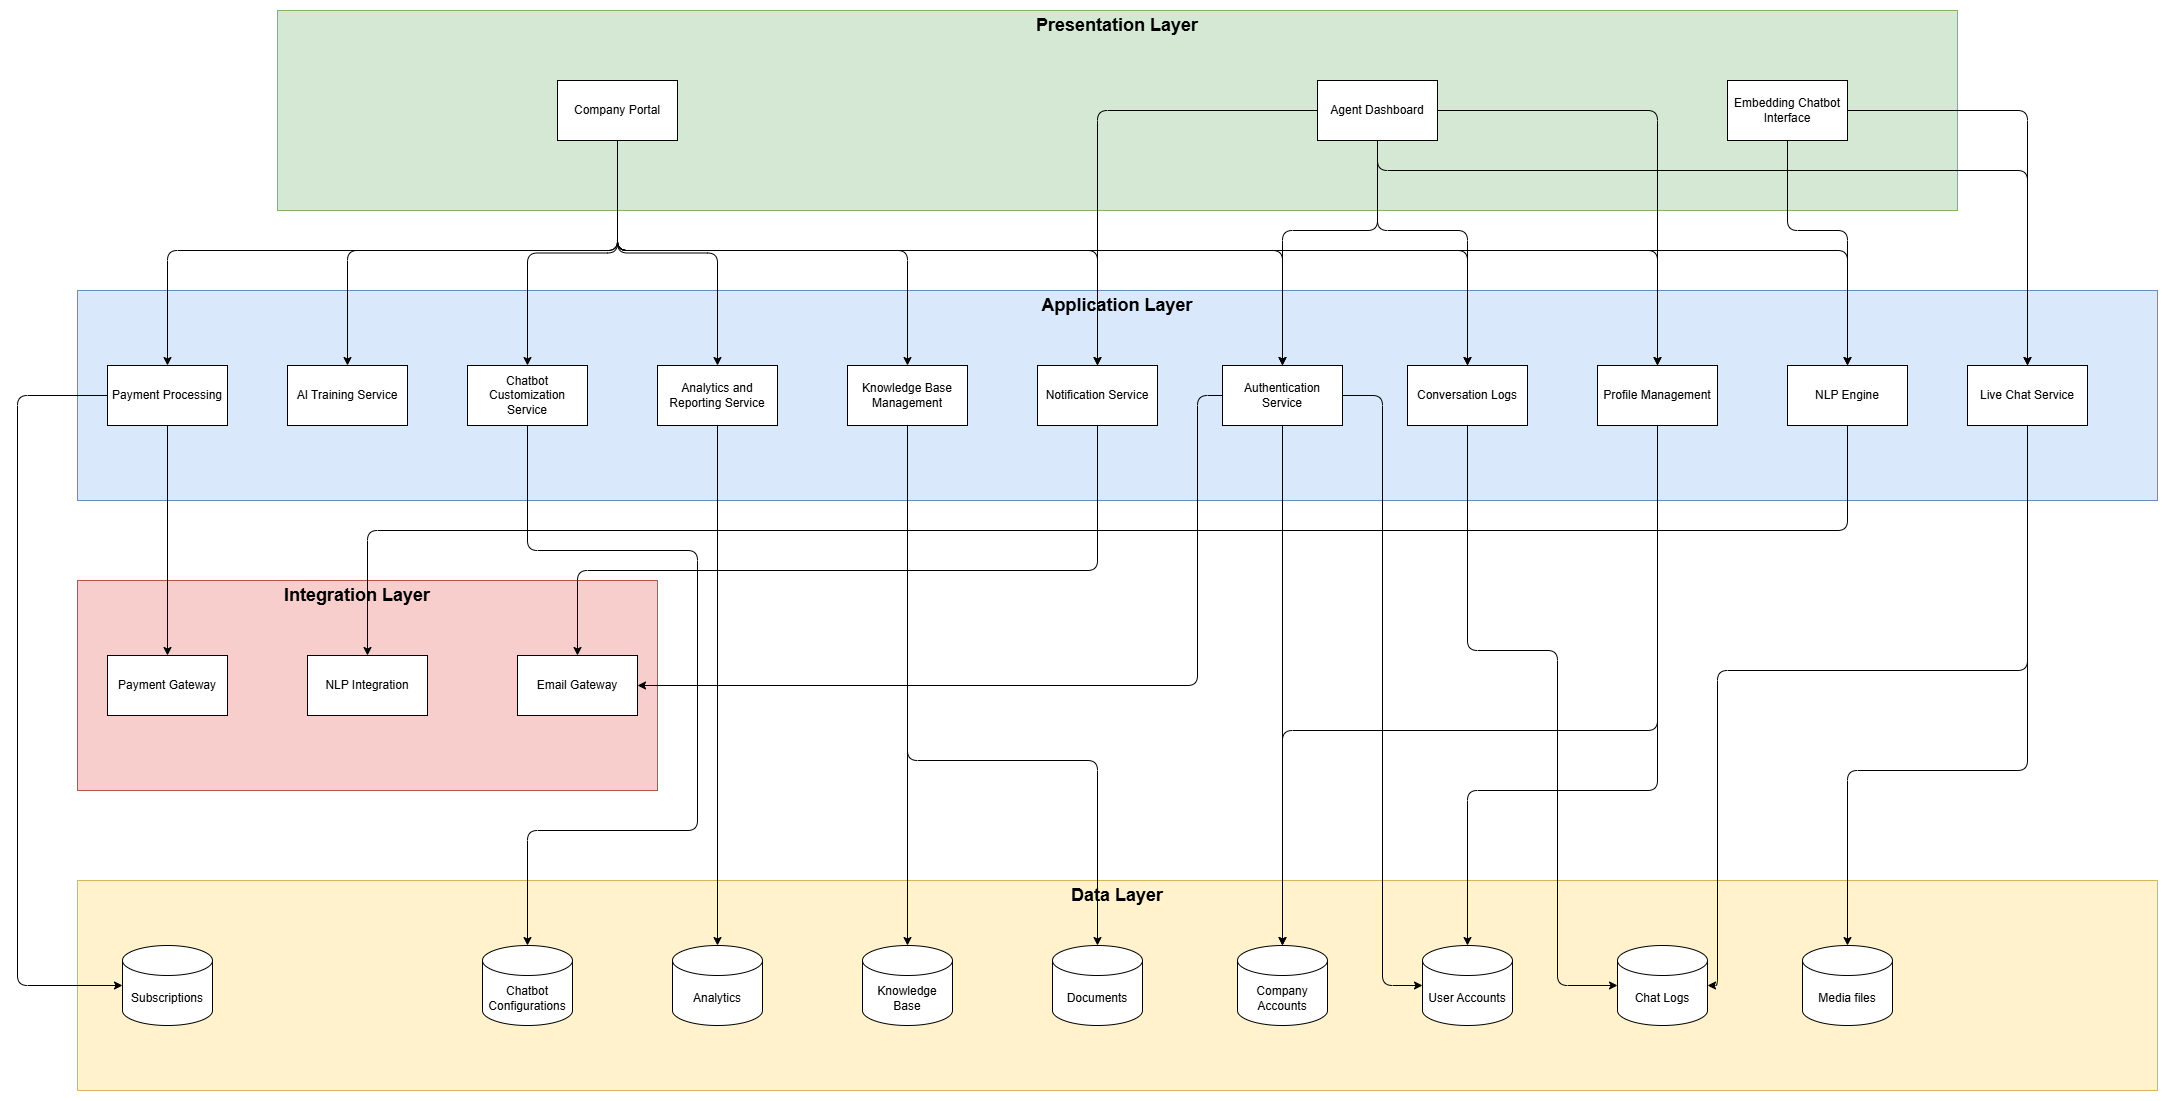
\includegraphics[height=0.9\textwidth, width=0.9\textheight, keepaspectratio]{Dg_System/system-architecture.png}
    }
    \rotatebox{90}{
        \parbox{\textwidth}{
            \centering
            \caption{Biểu đồ kiến trúc hệ thống}
            \label{fig:enter-label}
        }
    }
\end{figure}

\subsection{Kiến trúc hệ thống}
\subsubsection{Tổng quan kiến trúc}
Hệ thống được thiết kế dựa trên \textbf{kiến trúc nguyên khối có cấu trúc lớp (Layered Monolithic Architecture)} chủ đạo, kết hợp với các \textbf{thành phần xử lý bất đồng bộ} và tương tác với \textbf{dịch vụ AI nội bộ chuyên biệt được triển khai độc lập}. Trung tâm của hệ thống là một ứng dụng \textbf{Django} tập trung, đảm nhiệm vai trò xử lý các yêu cầu HTTP, triển khai logic nghiệp vụ cốt lõi và quản lý dữ liệu. Các thành phần chức năng chính được tổ chức dưới dạng các module dịch vụ bên trong ứng dụng nguyên khối này.

Lựa chọn kiến trúc này mang lại một số lợi ích chính. Thứ nhất, việc áp dụng kiến trúc nguyên khối cùng với hệ sinh thái toàn diện của Django cho phép \textbf{tối ưu hóa hiệu quả phát triển} và đẩy nhanh tốc độ triển khai tính năng. Thứ hai, hệ thống tích hợp \textbf{Django Channels (4.2)} và công nghệ \textbf{WebSocket} để đáp ứng yêu cầu giao tiếp thời gian thực, đặc biệt là cho chức năng trò chuyện, mà không đòi hỏi sự phức tạp của một kiến trúc phân tán hoàn toàn. Cuối cùng, mặc dù duy trì một lõi nguyên khối, kiến trúc vẫn đảm bảo \textbf{khả năng mở rộng} thông qua việc sử dụng \textbf{Celery} và \textbf{Redis} để xử lý các tác vụ nền và tác vụ định kỳ một cách bất đồng bộ, cho phép mở rộng quy mô của các tiến trình xử lý một cách độc lập khi tải tăng cao.

Giao tiếp với các ứng dụng phía người dùng được thực hiện chủ yếu thông qua \textbf{API Gateway} dựa trên \textbf{Django REST Framework} cho các yêu cầu REST API và \textbf{WebSocket Gateway} dựa trên Django Channels cho giao tiếp thời gian thực. Hệ thống được triển khai trên nền tảng \textbf{Heroku}, sử dụng \textbf{Gunicorn/Uvicorn} làm máy chủ WSGI/ASGI và \textbf{Whitenoise} để phục vụ các tệp tĩnh.
\subsubsection{Chi tiết các thành phần chính}

\subsubsubsection{Lớp ứng dụng (Application Layer)}
Trung tâm của hệ thống là ứng dụng Django đóng vai trò điều phối chính. Bên trong ứng dụng này, các chức năng nghiệp vụ được phân tách thành các module dịch vụ chuyên biệt, bao gồm:
\begin{itemize}
    \item \textbf{Module quản lý người dùng (User Service):} Chịu trách nhiệm xác thực, đăng ký, quản lý thông tin hồ sơ người dùng (bao gồm cả quản trị viên và nhân viên hỗ trợ), và thực thi cơ chế phân quyền truy cập trong toàn hệ thống.
    \item \textbf{Module quản lý tổ chức (Organization Service):} Quản lý cấu trúc nhóm/tổ chức, liên kết người dùng với tổ chức, và các quyền hạn, cài đặt riêng biệt áp dụng cho từng tổ chức sử dụng dịch vụ.
    \item \textbf{Module hội thoại (Chat Service):} Quản lý toàn bộ luồng giao tiếp thời gian thực trong hệ thống, bao gồm các cuộc hội thoại giữa người dùng cuối với \textbf{chatbot AI}, cũng như giữa người dùng cuối và \textbf{nhân viên hỗ trợ (human agents)}. Module này điều phối việc gửi/nhận tin nhắn qua WebSocket, quản lý trạng thái phiên chat, và có thể bao gồm logic phân phối chat cho nhân viên hoặc chuyển giao hội thoại giữa AI và người.
    \item \textbf{Module tùy chỉnh chatbot (Chatbot Service):} Chịu trách nhiệm cấu hình và vận hành các chatbot. Module này cho phép quản trị viên \textbf{tùy chỉnh} các khía cạnh của chatbot như giao diện hiển thị, hành vi, tính cách, và các kịch bản hội thoại cơ bản. Đồng thời, nó điều phối logic tương tác của chatbot trong cuộc hội thoại, phối hợp chặt chẽ với \textbf{dịch vụ AI} để thực hiện các tác vụ xử lý ngôn ngữ tự nhiên và sinh phản hồi thông minh.
    \item \textbf{Module xử lý tài liệu (Document Service):} Quản lý vòng đời của tài liệu tri thức được sử dụng bởi hệ thống và chatbot. Chức năng bao gồm tải lên, lưu trữ, phân loại, lập chỉ mục và truy xuất tài liệu. Quan trọng hơn, module này cung cấp logic để \textbf{kích hoạt quá trình huấn luyện} các mô hình AI dựa trên nội dung tài liệu được chọn lọc, đồng thời \textbf{theo dõi trạng thái} của các tiến trình huấn luyện này.
    \item \textbf{Module quản lý gói (Subscription Service):} Xử lý các nghiệp vụ liên quan đến thanh toán (tích hợp với PayOS) và quản lý các gói dịch vụ, bao gồm đăng ký, gia hạn, nâng cấp/hạ cấp gói, và theo dõi giới hạn sử dụng tài nguyên theo gói.
    \item \textbf{Module báo cáo (Report Service):} Thu thập dữ liệu từ các module khác để tổng hợp, phân tích và \textbf{tạo ra các báo cáo} chi tiết về hiệu suất hoạt động, cung cấp thông tin giá trị cho việc đánh giá và cải tiến hệ thống.
\end{itemize}
Cách tổ chức theo module này, tận dụng cấu trúc ứng dụng của Django, giúp duy trì sự tách biệt rõ ràng về chức năng trong một mã nguồn thống nhất, thuận lợi cho việc phát triển, kiểm thử và bảo trì.


\subsubsubsection{Lớp giao tiếp (Interface Layer)}
\begin{itemize}
    \item \textbf{API Gateway:} Được xây dựng trên nền tảng Django REST Framework, cung cấp giao diện REST API chuẩn hóa cho các frontend tương tác với backend.
    \item \textbf{WebSocket Gateway:} Sử dụng Django Channels, thiết lập kênh giao tiếp hai chiều, thời gian thực, chủ yếu phục vụ cho tính năng trò chuyện.
\end{itemize}

\subsubsubsection{Xử lý tác vụ nền (Background Processing)}
\begin{itemize}
    \item \textbf{Celery Workers:} Các tiến trình độc lập thực thi các tác vụ tốn thời gian hoặc tài nguyên một cách bất đồng bộ, giúp giải phóng luồng xử lý chính của ứng dụng web và cải thiện độ phản hồi.
    \item \textbf{Redis Message Queue:} Đóng vai trò là hàng đợi tin nhắn, trung gian giao tiếp giữa ứng dụng Django và các Celery workers.
\end{itemize}

\subsubsubsection{Lớp dữ liệu (Data Layer)}
\begin{itemize}
    \item \textbf{PostgreSQL:} Hệ quản trị cơ sở dữ liệu quan hệ chính, lưu trữ hầu hết dữ liệu có cấu trúc của hệ thống như thông tin người dùng, tổ chức, lịch sử trò chuyện, cấu hình chatbot, thông tin thuê bao, và dữ liệu tài liệu.
    item \textbf{Redis:} Đóng vai trò đa năng quan trọng trong hệ thống, phục vụ ba mục đích chính:
        \begin{itemize}
            \item Làm \textbf{bộ nhớ đệm} để tối ưu hóa tốc độ truy xuất các dữ liệu thường dùng.
            \item Làm \textbf{backend cho lớp channels} của Django Channels, hỗ trợ việc quản lý và truyền tải tin nhắn hiệu quả cho giao tiếp thời gian thực qua WebSocket.
            \item Làm \textbf{hàng đợi tin nhắn} cho hệ thống xử lý tác vụ nền Celery, điều phối việc thực thi các tác vụ bất đồng bộ.
        \end{itemize}
\end{itemize}

\subsubsubsection{Dịch vụ AI}
Hệ thống bao gồm một dịch vụ AI chuyên biệt, triển khai độc lập và tách biệt với backend. Dịch vụ này chuyên trách việc cung cấp các khả năng xử lý ngôn ngữ tự nhiên và trí tuệ đối thoại tiên tiến, tận dụng các mô hình ngôn ngữ lớn. Module chat bên trong ứng dụng lõi sẽ giao tiếp với Dịch vụ AI này thông qua giao diện REST API.

Việc lựa chọn triển khai Dịch vụ AI một cách độc lập mang lại một số lợi ích về mặt kiến trúc và vận hành:
\begin{itemize}
    \item \textbf{Tối ưu tài nguyên:} Cho phép dịch vụ AI chạy trên hạ tầng phần cứng chuyên biệt và được cấp phát tài nguyên tối ưu cho các tác vụ tính toán nặng của AI.
    \item \textbf{Khả năng mở rộng độc lập:} Quy mô của Dịch vụ AI có thể được điều chỉnh một cách linh hoạt dựa trên tải xử lý AI, độc lập với việc mở rộng quy mô của ứng dụng web lõi.
    \item \textbf{Linh hoạt về công nghệ và cập nhật:} Cho phép sử dụng các thư viện, framework, hoặc thậm chí ngôn ngữ lập trình khác (phù hợp hơn cho AI/ML) và có thể cập nhật các mô hình AI thường xuyên mà không cần phải triển khai lại toàn bộ ứng dụng lõi.
    \item \textbf{Tách biệt lỗi:} Sự cố tiềm ẩn trong dịch vụ AI ít có khả năng ảnh hưởng trực tiếp đến sự ổn định của ứng dụng web chính và ngược lại.
\end{itemize}

\subsubsubsection{Tích hợp dịch vụ bên ngoài}
Ngoài các thành phần nội bộ, hệ thống còn tích hợp với các dịch vụ của bên thứ ba chuyên biệt để mở rộng chức năng và tận dụng các giải pháp đã được tối ưu hóa trên thị trường:
\begin{itemize}
    \item \textbf{AWS S3 (Simple Storage Service):} Dịch vụ lưu trữ đối tượng trên nền tảng đám mây của Amazon Web Services, được sử dụng để lưu trữ bền vững và có khả năng mở rộng cao cho các tệp tài liệu, hình ảnh, video và các dữ liệu media khác do người dùng tải lên hoặc hệ thống tạo ra.
    \item \textbf{PayOS:} Một cổng thanh toán của bên thứ ba, cung cấp giao diện và xử lý các giao dịch thanh toán trực tuyến một cách an toàn, hỗ trợ nhiều phương thức thanh toán khác nhau, phục vụ cho việc quản lý đăng ký và thuê bao dịch vụ.
    \item \textbf{SendGrid:} Dịch vụ chuyên dụng cho việc gửi email, đảm bảo khả năng gửi email giao dịch (ví dụ: xác nhận đăng ký, đặt lại mật khẩu) và email thông báo đến người dùng với tỉ lệ gửi thành công cao và tuân thủ các tiêu chuẩn về email.
\end{itemize}

Tóm lại, kiến trúc nguyên khối có cấu trúc lớp này cân bằng giữa hiệu quả phát triển, khả năng bảo trì và các yêu cầu về hiệu năng, thời gian thực. Việc tích hợp các thành phần xử lý bất đồng bộ và các dịch vụ bên ngoài chuyên biệt giúp hệ thống giải quyết các bài toán phức tạp về xử lý nền, lưu trữ và trí tuệ nhân tạo mà vẫn duy trì được sự đơn giản tương đối trong cấu trúc lõi.

\subsection{Giao diện}
\subsubsection{Lược đồ Screen-flow}
Lược đồ này cung cấp cái nhìn tổng quan về trải nghiệm người dùng: cách các trang giao diện kết nối với nhau, thứ tự hiển thị, và ai là người kiểm soát trang giao diện đó (phân chia vai trò). Cụ thể, quản trị viên và các nhân viên chăm sóc khách hàng quản lý hầu hết các trang, và người dùng khi tiếp cận với trang web doanh nghiệp, chỉ cần tương tác với chatbot popup là đủ.

\begin{figure}[H]
	\centering
	\includesvg[width=\textwidth]{Figma/Screens-Flow-Diagram.svg}
	\vspace{0.5cm}
	\caption{Lược đồ Screen-flow}
	\label{fig:enter-label}
\end{figure}

\subsubsection{Logo ứng dụng}

\begin{figure}[H]
	\centering
	
\includegraphics[width=0.4\textwidth]{Figma/logo.png}
	\vspace{0.5cm}
	\caption{Logo của ứng dụng CoolChat}
	\label{fig:enter-label}
\end{figure}

% Định dạng tùy chỉnh a), b), c)
\renewcommand{\labelenumi}{\alph{enumi})}

\begin{enumerate}
	\item \textbf{Tên ứng dụng}
	\begin{itemize}
		\item Ứng dụng được triển khai có tên là CoolChat.
		\item CoolChat hướng đến việc trở thành thương hiệu số 1 Việt Nam trong công cuộc đồng hành cùng các doanh nghiệp trên hành trình tư vấn và chăm sóc khách hàng của họ.
	\end{itemize}
	
	\item \textbf{Biểu tượng}
	
	Đây là hình ảnh logo đầy đủ của hệ thống cung cấp chatbot CoolChat.
	\begin{itemize}
		\item Logo là hình ảnh một biểu tượng chatbot được cách điệu một cách hiện đại và trẻ trung. Màu xanh dương được sử dụng làm màu chủ đạo, mang đến cảm giác tươi mát, tin cậy và chuyên nghiệp.
		\item Slogan "Make it cool": CoolChat cam kết mang đến những trải nghiệm giao tiếp thú vị và mới mẻ cho người dùng trong lĩnh vực giao tiếp và tư vấn trực tuyến.
	\end{itemize}
	
\end{enumerate}

% Trở về định dạng mặc định 1., 2., 3.
\renewcommand{\labelenumi}{\arabic{enumi}.}


\subsubsection{Trang Đích}
\begin{figure}[H]
    \centering
    \fbox{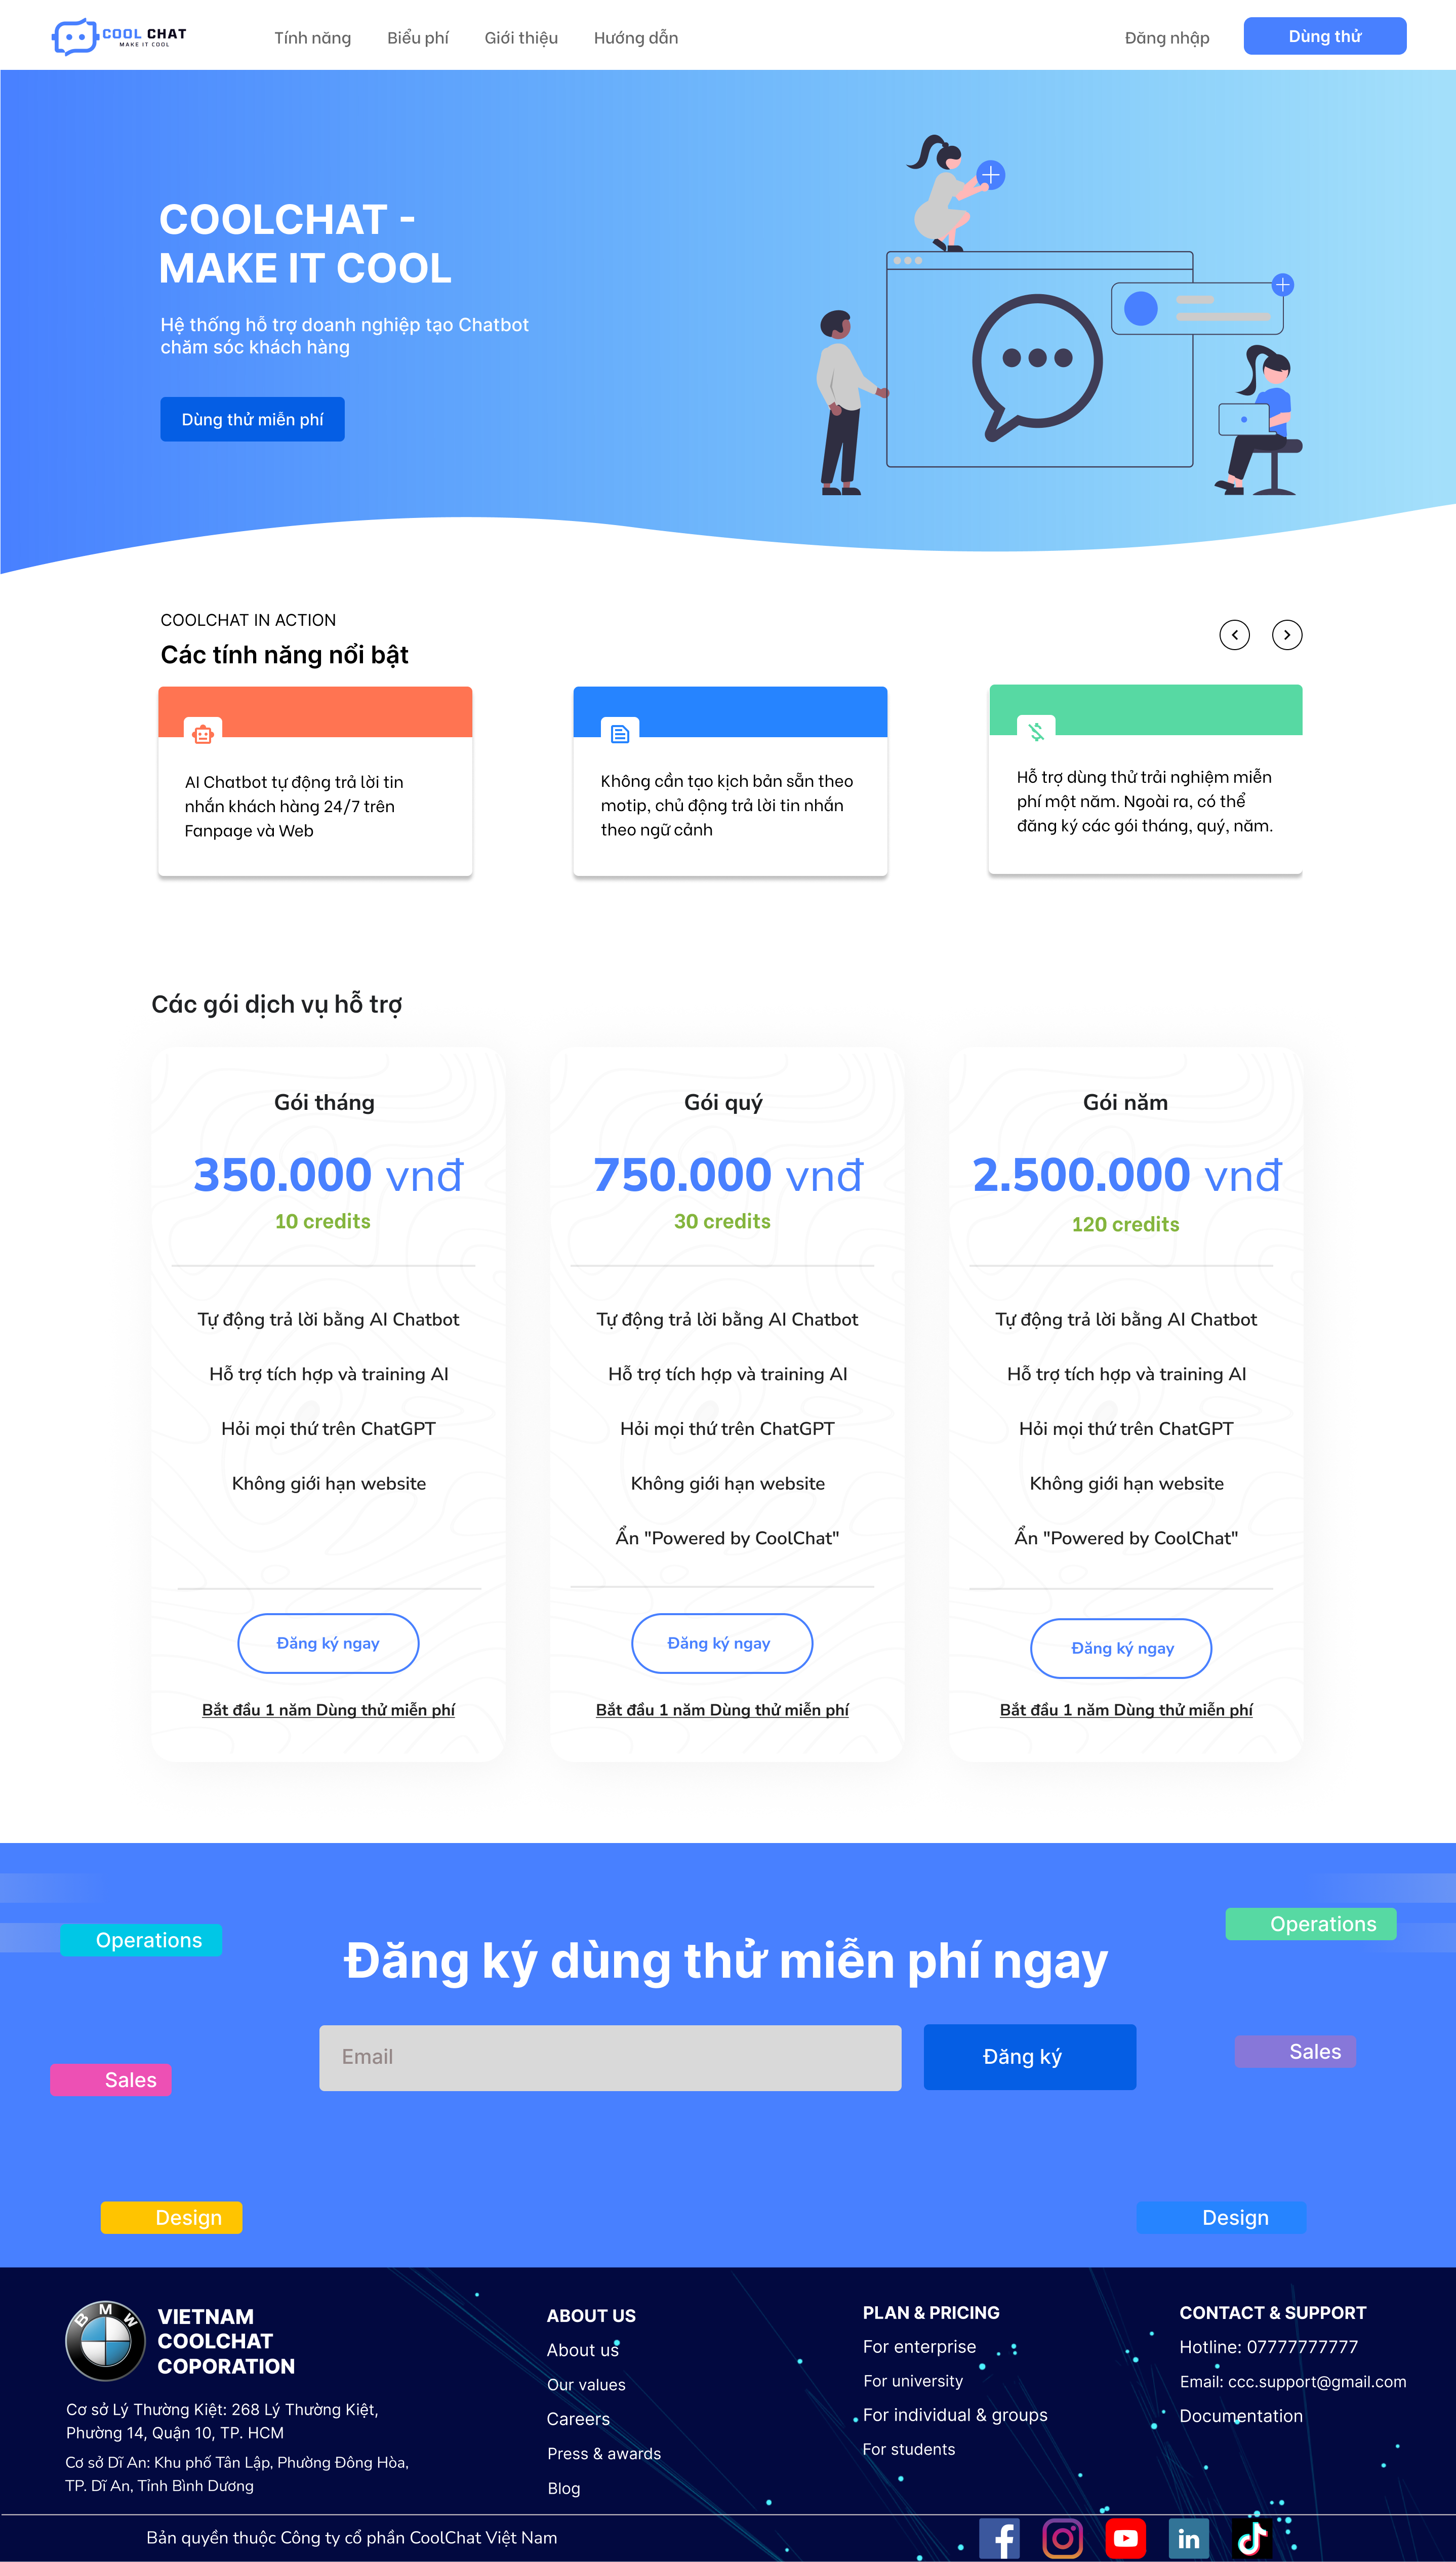
\includegraphics[width=0.75\linewidth]{Figma/landing.png}}
    \vspace{0.5cm}
    \caption{Giao diện trang Đích}
    \label{fig:enter-label}
\end{figure}

Giao diện Trang đích cung cấp một giao diện tổng thể giúp doanh nghiệp tiếp cận được những thông tin quan trọng và cần thiết nhất của hệ thống. Giao diện gồm các phần:

% Định dạng tùy chỉnh a), b), c)
\renewcommand{\labelenumi}{\alph{enumi})}

\begin{enumerate}
	\item \textbf{Thanh header}
	Bao gồm một Logo của hệ thống và các nút điều hướng đến các phần Nội dung và điều hướng đến trang đăng nhập và đăng ký.
	\item \textbf{Nội dung}
	Phần nội dung được chia làm các phần nhỏ:
	\begin{itemize}
		\item Phần Chào đón: bao gồm câu khẩu hiệu, nút Dùng thử miễn phí và một slider các hình ảnh cùng với phông nền màu xanh đăng trưng.
		\item Phần Các tính năng nổi bật: bao gồm một slider để hiển thị các tính năng đặc trưng và tiêu biểu của hệ thống, giúp người dùng nhận diện và tiếp cận một cách nhanh nhất. 
		\item Phần Biểu phí: hiển thị các gói đăng ký mà hệ thống hỗ trợ, người dùng có thể bấm nút đăng ký gói hoặc nút đăng ký dùng thử miễn phí.
		\item Phần Đăng ký: đây là phần giúp người dùng có thể điền email và chuyển đến trang đăng ký.
	\end{itemize}
	\item \textbf{Thanh footer}
	Thanh footer là thanh nằm cuối cùng của hệ thống với các phần sau:
	\begin{itemize}
		\item Phần Logo và địa chỉ: cung cấp hình ảnh logo công ty và địa chỉ các chi nhánh của công ty.
		\item Phần Giới thiệu: bao gồm các nút điều hướng đến các thông tin liên quan đến công ty như giới thiệu, giá trị, tuyển dụng, giải thưởng và blog.
		\item Phần Biểu phí: hiển thị các loại biếu phí hỗ trợ như doanh nghiệp, trường đại học, cá nhân và nhóm và sinh viên.
		\item Phần Liên hệ: hiển thị số hotline, địa chỉ email cũng như các liên kết đến các nền tảng xã hội của công ty.
		\item Phần Bản quyền: hiển thị chủ sở hữu bản quyền hệ thống.
	\end{itemize}
\end{enumerate}

% Trở về định dạng mặc định 1., 2., 3.
\renewcommand{\labelenumi}{\arabic{enumi}.}

\subsubsection{Trang Đăng ký}
\setlength{\fboxsep}{0pt}
\begin{figure}[H]
	\centering
	\fbox{\includesvg[width=\textwidth]{Figma/Signup - STEP 1.svg}}
	\vspace{0.5cm}
	\caption{Giao diện trang Đăng ký}
	\label{fig:enter-label}
\end{figure}

Giao diện Đăng ký cung cấp một biểu mẫu để người dùng điền các thông tin cá nhân cần thiết và đặt mật khẩu cho tài khoản. Bố cục của trang đơn giản và chia làm 3 phần chính:

% Định dạng tùy chỉnh a), b), c)
\renewcommand{\labelenumi}{\alph{enumi}}

\begin{enumerate}
	\item \textbf{Tiêu đề}
	\begin{itemize}
		\item Logo của ứng dụng được đặt lên đầu tiên nhằm khắc ghi nhận diện thương hiệu vào tâm trí người dùng.
		\item Phần lời dẫn nhằm giới thiệu mục tiêu của ứng dụng và nhấn mạnh sự tiện lợi CoolChat đem lại khi người sử dụng tiếp cận.
	\end{itemize}
	
	\item \textbf{Biểu mẫu}
	\begin{itemize}
		\item Cho phép người dùng điền các thông tin cá nhân cần thiết: tên, số điện thoại, email doanh nghiệp, vai trò.
		\item Yêu cầu người dùng đặt mật khẩu và xác nhận mật khẩu lần nữa.
		\item Đề nghị người dùng đồng ý với các điều khoản và chính sách khi sử dụng dịch vụ.
	\end{itemize}
	
	\item \textbf{Điều hướng}
	\begin{itemize}
		\item Nút màu xanh 'Tạo tài khoản mới' giúp người dùng hoàn thành bước đăng ký sau khi đã điền xong biểu mẫu.
		\item Người dùng có thể điều hướng sang trang đăng nhập nếu đã có sẵn tài khoản trước đó.
	\end{itemize}
	
\end{enumerate}

% Trở về định dạng mặc định 1., 2., 3.
\renewcommand{\labelenumi}{\arabic{enumi}.}


\subsubsection{Trang Đăng nhập}

\begin{figure}[H]
	\centering
	\fbox{\includesvg[width=\textwidth]{Figma/Login.svg}}
	\vspace{0.5cm}
	\caption{Giao diện trang Đăng nhập}
	\label{fig:enter-label}
\end{figure}

Giao diện Đăng nhập cung cấp cho người sử dụng nhiều phương thức khác nhau để truy cập tài khoản. Cụ thể:
\begin{itemize}
	\item Qua Google nếu tài khoản của bạn có vai trò admin.
	\item Qua Google nếu tài khoản của bạn có vai trò nhân viên chăm sóc khách hàng.
	\item Qua tài khoản và mật khẩu.
\end{itemize}

Với cách thức thứ ba, người dùng có thể lấy lại mật khẩu qua lựa chọn 'Quên mật khẩu' bên dưới ô nhập email. Ngoài ra, người sử dụng cũng quay về được trang Đăng ký nếu muốn.

\subsubsection{Trang Đào tạo chatbot}
Giao diện này gồm hai tiểu phần: Gán nhãn tri thức và cập nhật tri thức.
\subsubsubsection{Gán nhãn tri thức}

\begin{figure}[H]
	\centering
	\fbox{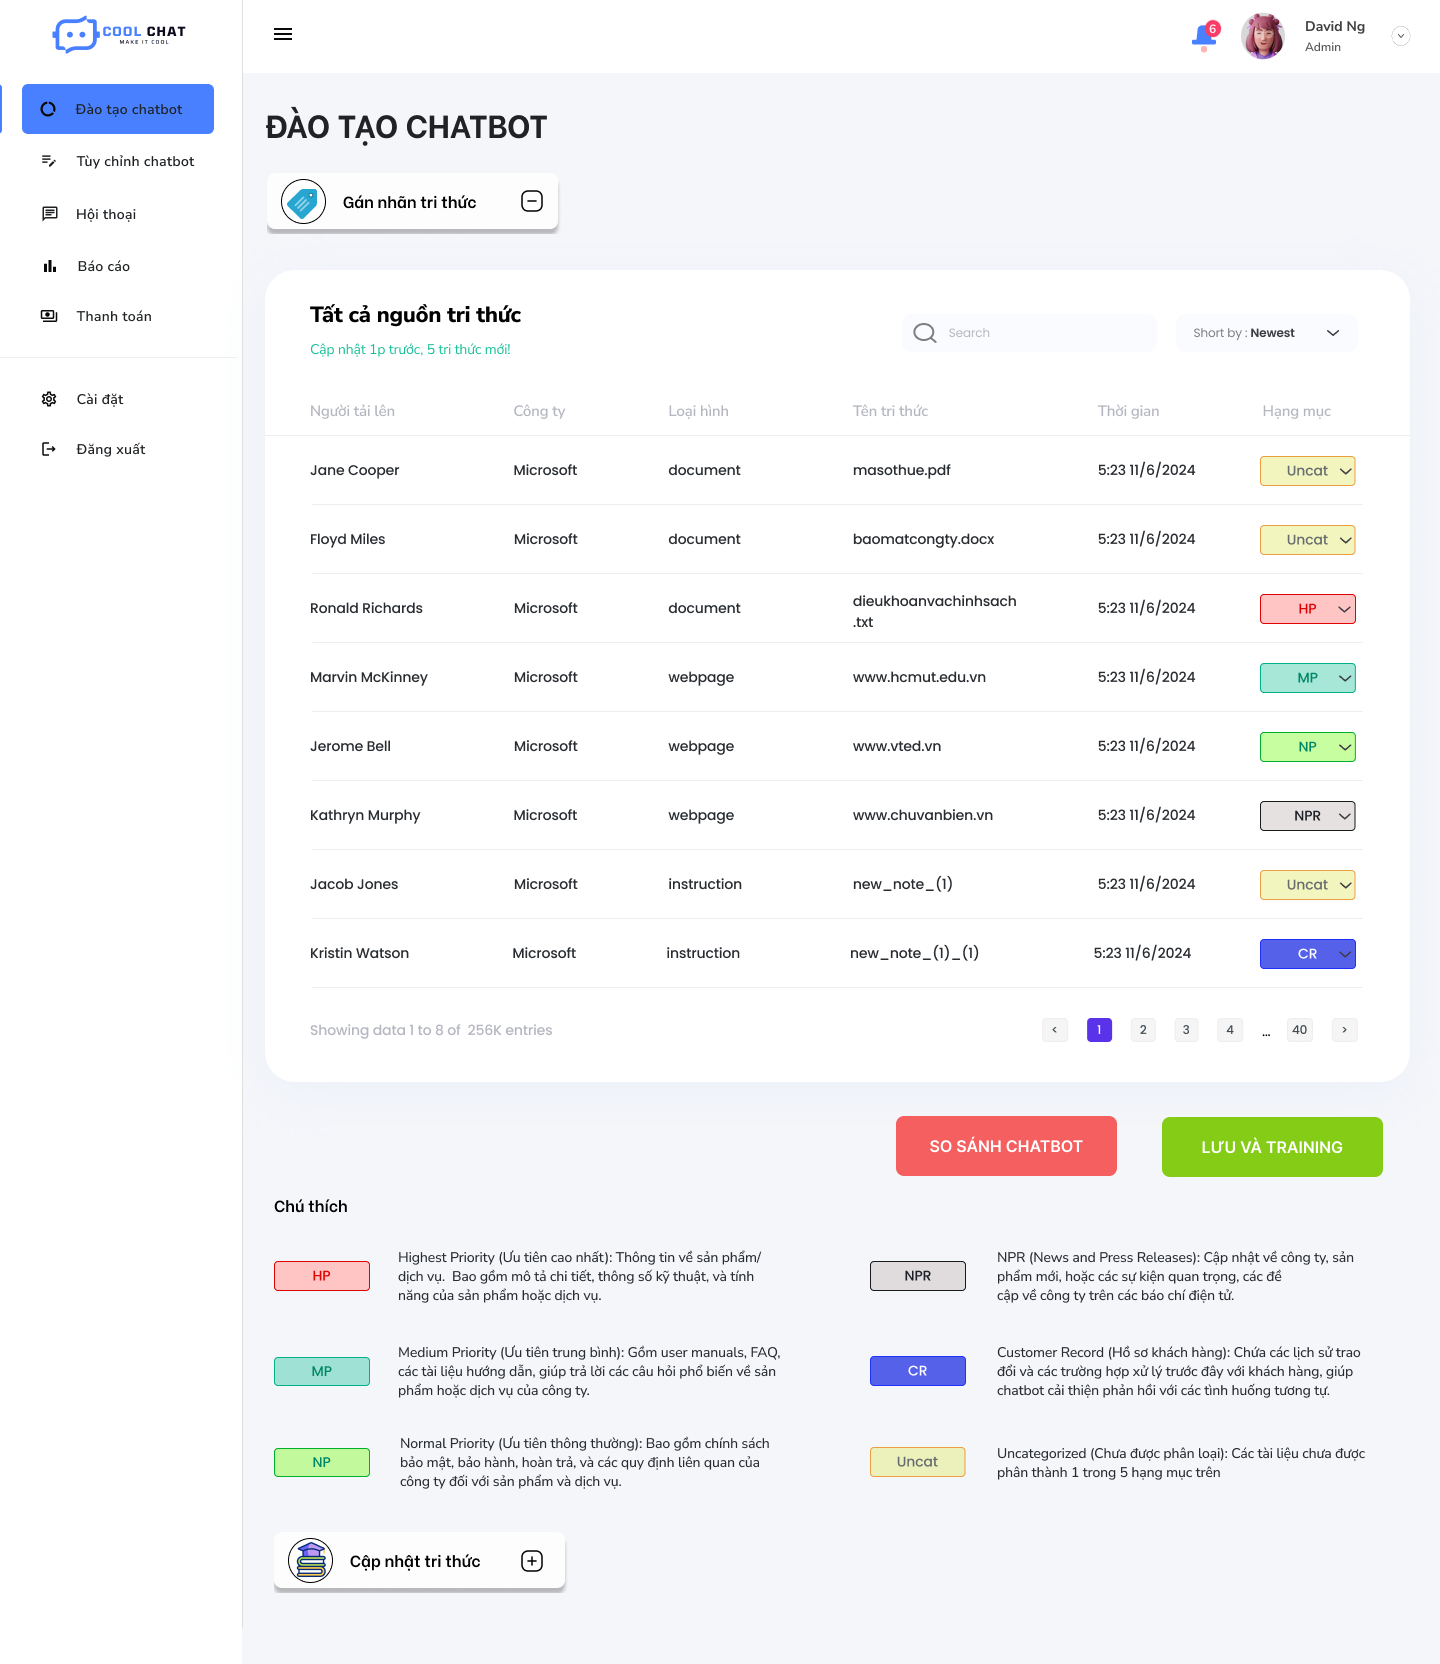
\includegraphics[width=\textwidth]{Figma/GNTT.png}}
	\vspace{0.5cm}
	\caption{Giao diện mục Gán nhãn tri thức}
	\label{fig:enter-label}
\end{figure}

Giao diện Gán nhãn tri thức cung cấp cho người sử dụng một bảng liệt kê các tài liệu tri thức dành cho chatbot. Các chú thích dành cho quản trị viên nằm ở bên dưới - cung cấp thông tin ưu tiên thứ tự truy xuất cho chatbot khi trả lời một câu hỏi. Hai nút thao tác:
\begin{itemize}
	\item So sánh chatbot (màu đỏ): sử dụng khi quản trị viên muốn so sánh câu trả lời của chatbot cũ và mới (do thay đổi tài liệu, thứ tự ưu tiên, phong cách trả lời...) 
	\item Lưu và training (màu xanh): nhấn nút này khi quản trị viên muốn cập nhật và training ngay chatbot mà không cần so sánh.
\end{itemize}
\begin{figure}[H]
	\centering
	\fbox{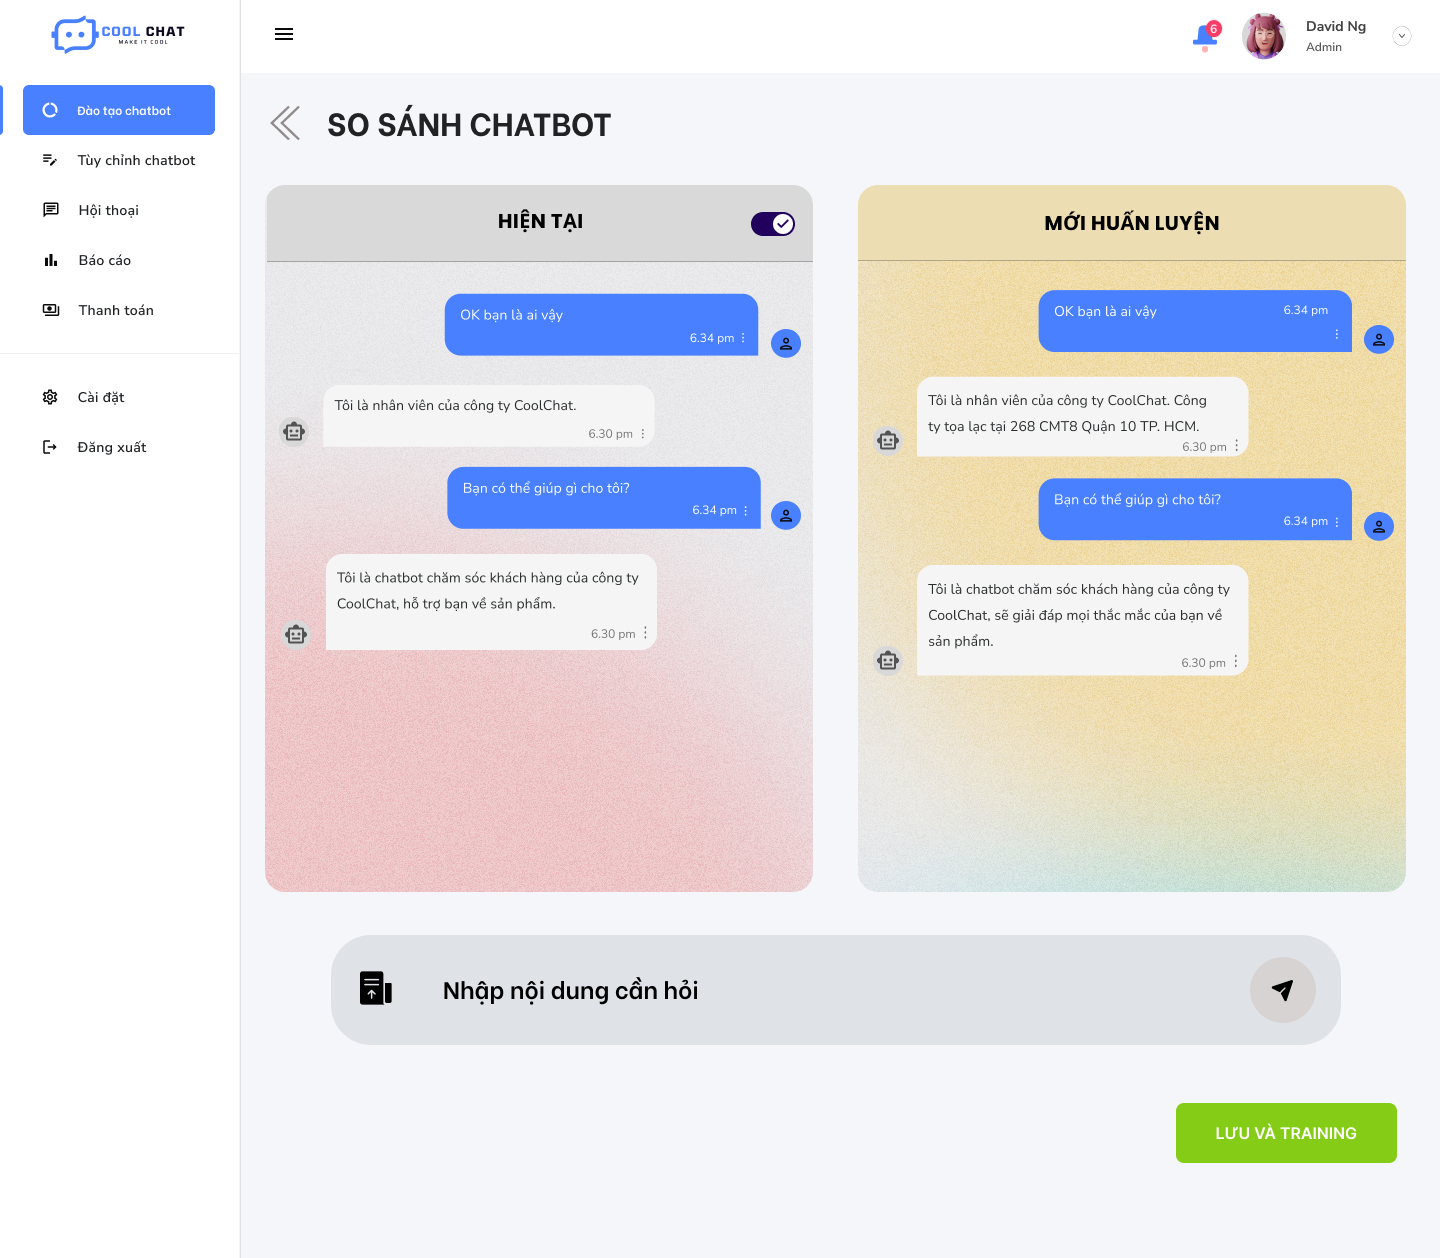
\includegraphics[width=\textwidth]{Figma/SSCB.png}}
	\vspace{0.5cm}
	\caption{Giao diện trang So sánh chatbot}
	\label{fig:enter-label}
\end{figure}

\subsubsubsection{Cập nhật tri thức}
Giao diện Cập nhật tri thức cung cấp cho người sử dụng nhiều phương thức để thêm, xóa, sửa tài liệu tri thức dành cho chatbot. Hiện tại CoolChat hỗ trợ ba phương tiện tri thức:
\begin{itemize}
	\item Tệp (mục Tải lên phương tiện): hỗ trợ các loại tệp pdf, doc, docx, và txt.
	\item Nhập từ bàn phím (ô Nhập tri thức): tự nhập hướng dẫn cho chatbot, sau đó các hướng dẫn sẽ được lưu ở dạng txt.
	\item Trích xuất từ web (ô Nhập tri thức web): cần thiết khi không có sẵn tài liệu hoặc muốn lấy thông tin từ một trang web cụ thể.
\end{itemize}

\begin{figure}[H]
	\centering
	\fbox{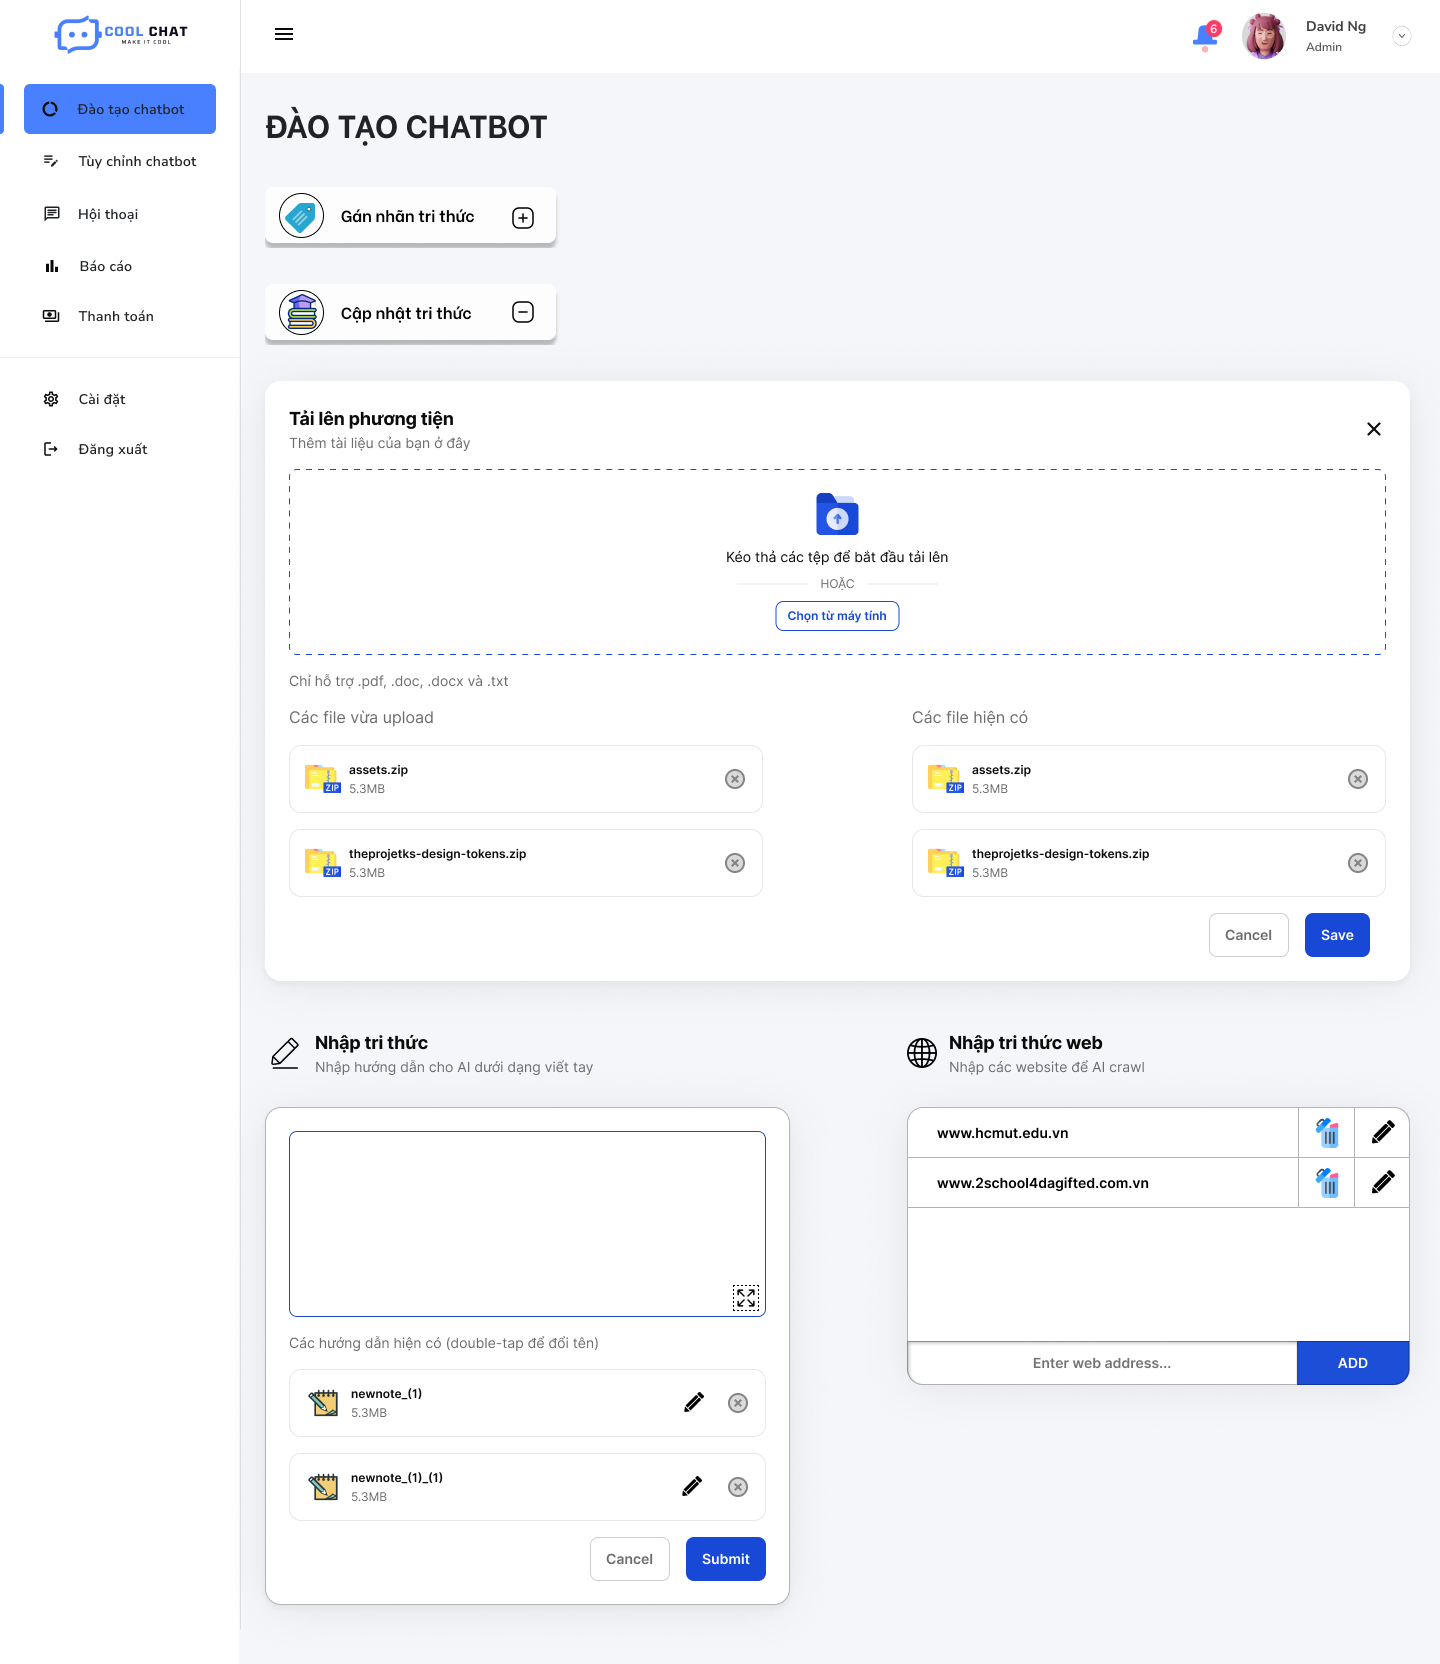
\includegraphics[width=\textwidth]{Figma/GNTT2.png}}
	\vspace{0.5cm}
	\caption{Giao diện mục Cập nhật tri thức}
	\label{fig:enter-label}
\end{figure}

\subsubsection{Trang Tùy chỉnh chatbot}
Giao diện này gồm hai tiểu phần: Cấu hình hiển thị và tích hợp AI.
\subsubsubsection{Cấu hình hiển thị}

\begin{figure}[H]
	\centering
	\fbox{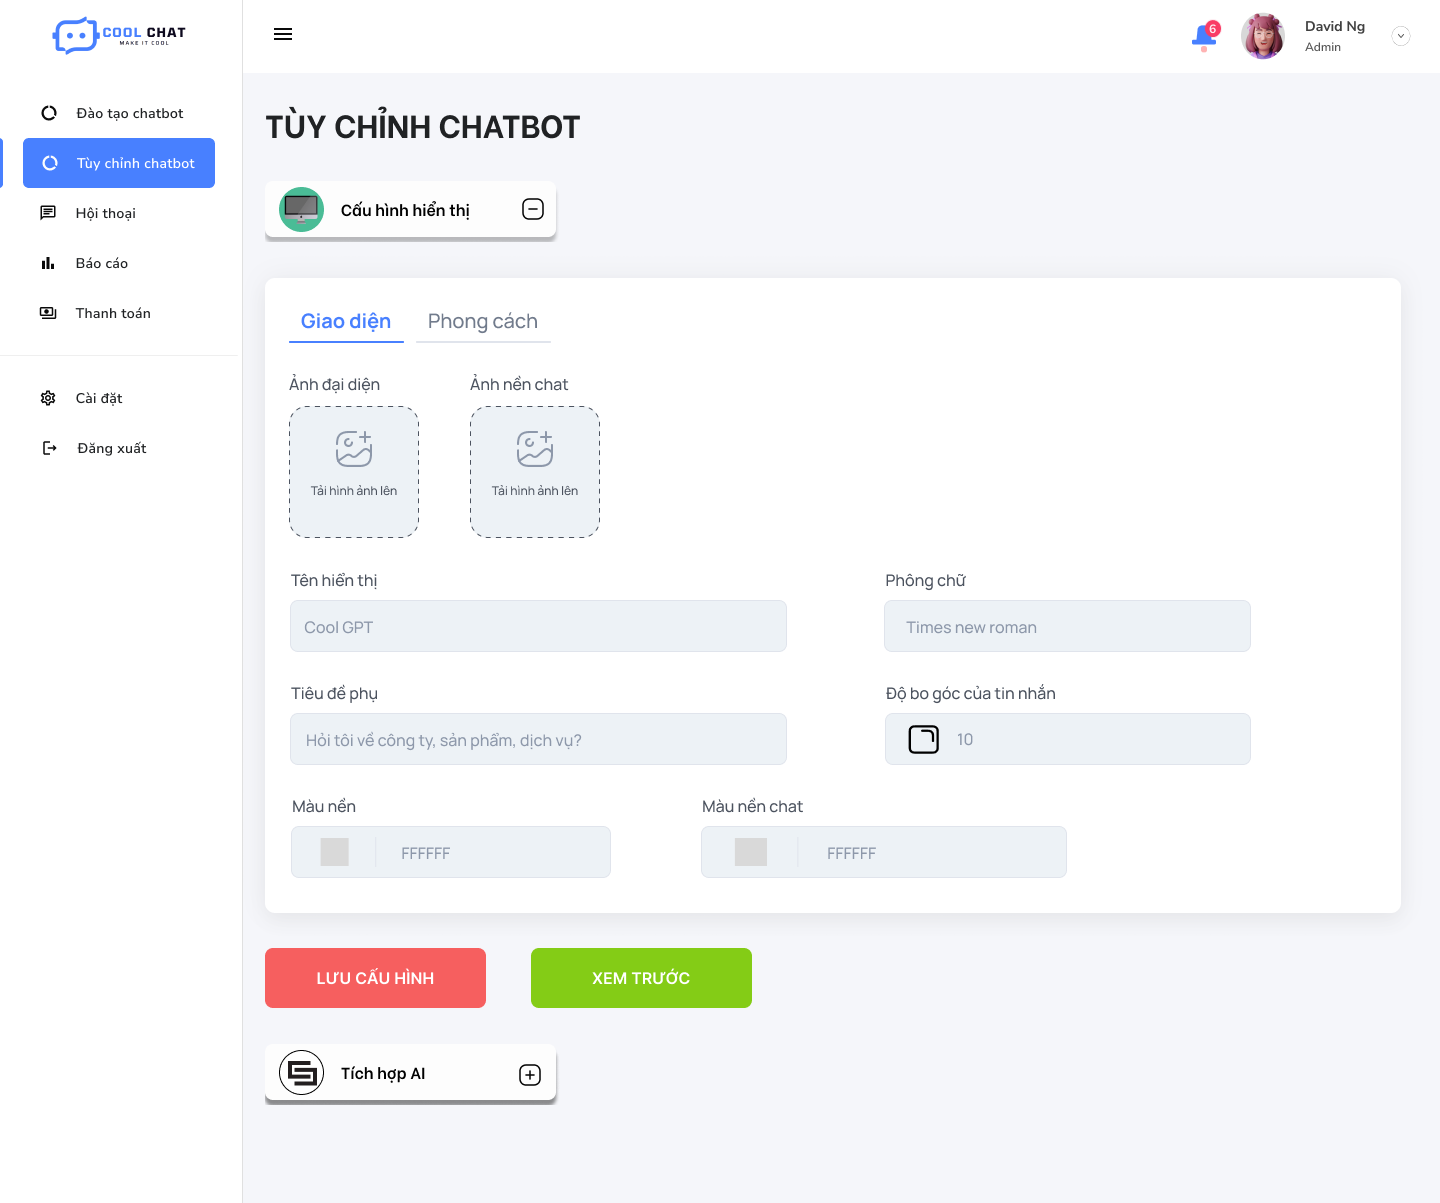
\includegraphics[width=\textwidth]{Figma/CHHT1.png}}
	\vspace{0.5cm}
	\caption{Giao diện mục Cấu hình hiển thị - Giao diện}
	\label{fig:enter-label}
\end{figure}

Giao diện Cấu hình hiển thị cung cấp cho người sử dụng giao diện động linh hoạt chuyển đổi giữa hai loại cấu hình: Giao diện (Hình 73) và Phong cách (Hình 74). 
\begin{itemize}
	\item Về giao diện: ảnh đại diện, ảnh nền chat, tên hiển thị, phông chữ, tiêu đề phụ, độ bo góc của tin nhắn, màu nền, màu nền chat đều là các yếu tố có thể thay đổi bởi quản trị viên. Điều này mục đích tạo điểm nhấn và nhận diện thương hiệu trong mắt khách hàng.
	
	Quản trị viên hoàn toàn xem trước được cấu hình (nút màu xanh "Xem trước") sau đó nhấn "Lưu cấu hình" (nút màu đỏ).
	\item Về phong cách: Tạo ra trải nghiệm riêng biệt về doanh nghiệp trong quá trình tư vấn thông qua:
	\begin{itemize}
		\item Tông giọng bot: có 4 tông giọng có sẵn, và có thể nhiều hơn trong tương lai.
		\item Tin nhắc mặc định: lời chào đầu, lời tạm biệt, và lời chuyển giao. 
	\end{itemize}
	
	Quản trị viên có thể xem chatbot ngay tại giao diện này sau khi lưu các thay đổi bằng nút "Xem chatbot".
\end{itemize}
\begin{figure}[H]
	\centering
	\fbox{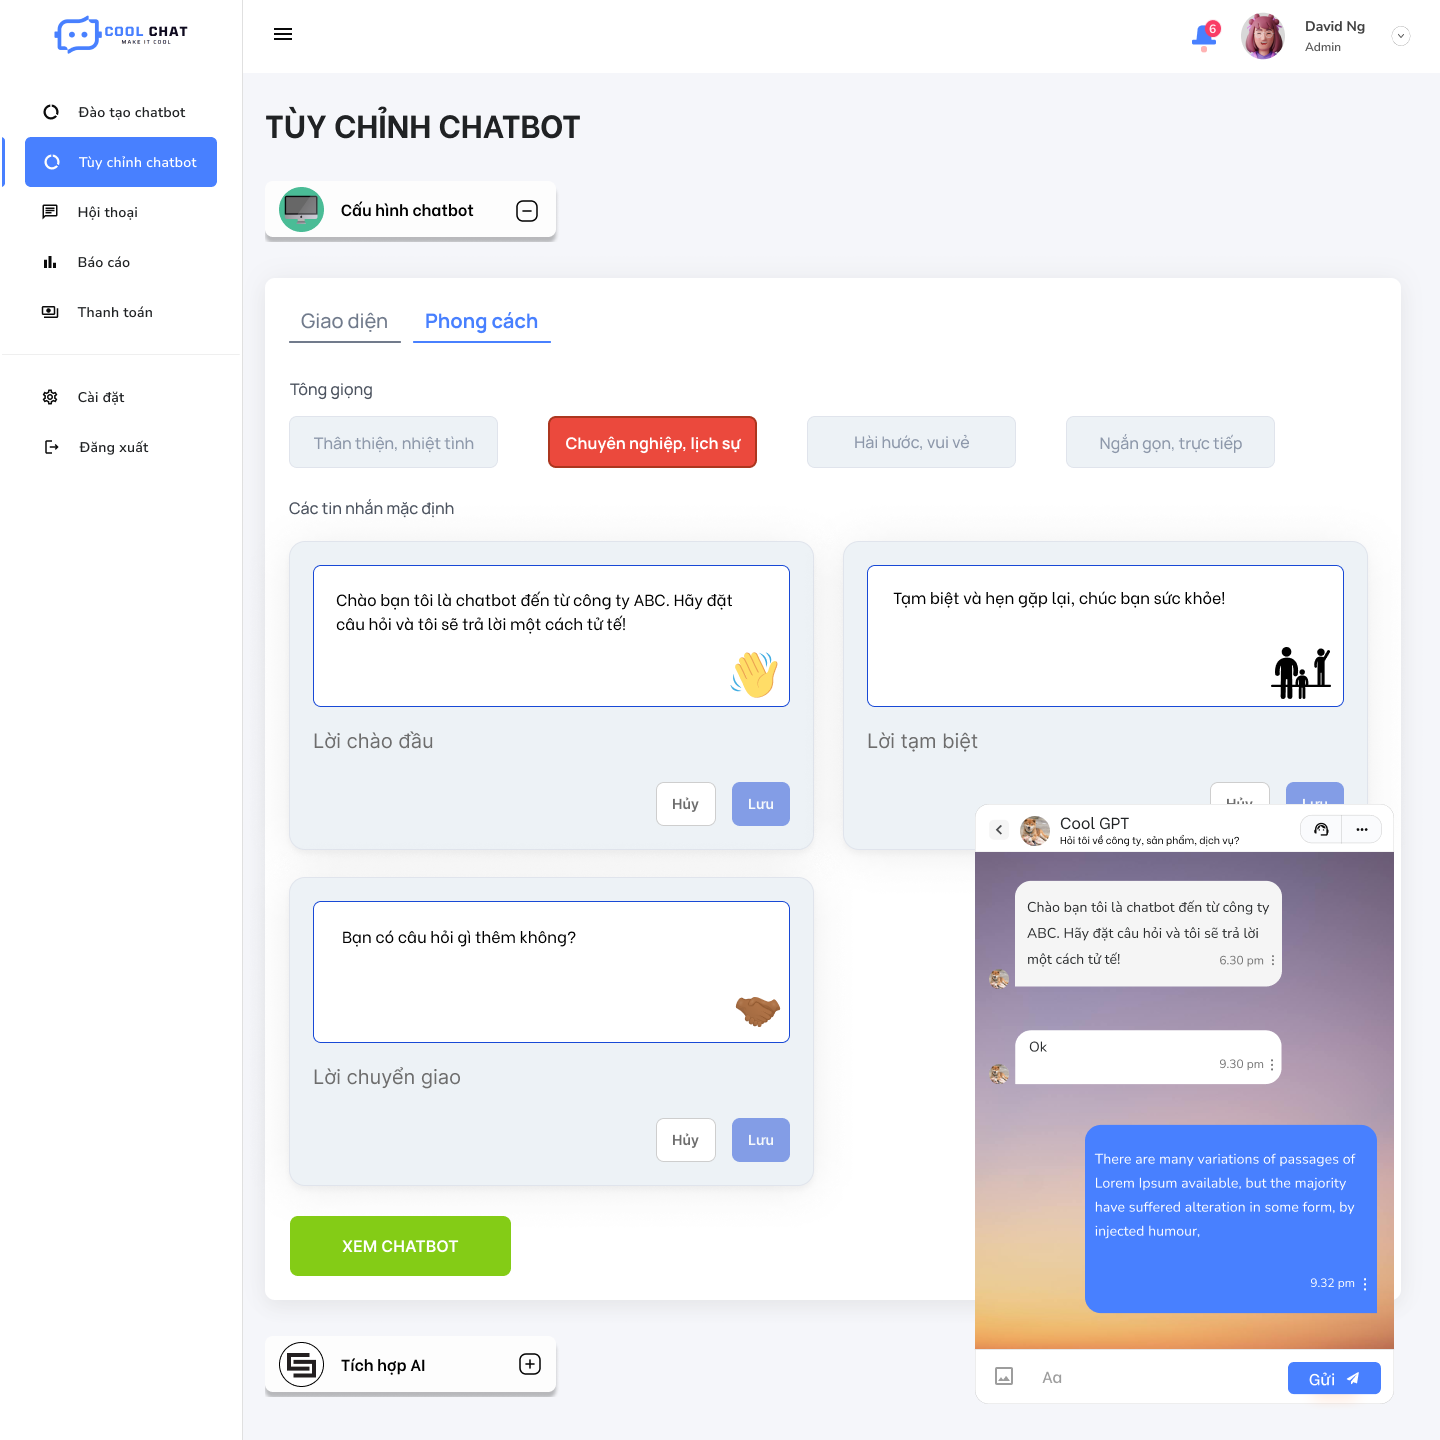
\includegraphics[width=\textwidth]{Figma/CHHT2.png}}
	\vspace{0.5cm}
	\caption{Giao diện mục Cấu hình hiển thị - Phong cách}
	\label{fig:enter-label}
\end{figure}

\subsubsubsection{Tích hợp AI}
Chatbot có thể kết nối được với nền tảng mạng xã hội (facebook chính thức của doanh nghiệp) hoặc trang web đều được. 
\begin{itemize}
	\item Kết nối facebook: Qua nút "Kết nối tới facebook".
	\item Kết nối trang web: Sao chép mã nguồn từ tab mã nhúng và đưa vào mã nguồn trang web của doanh nghiệp.
\end{itemize}

\begin{figure}[H]
	\centering
	\fbox{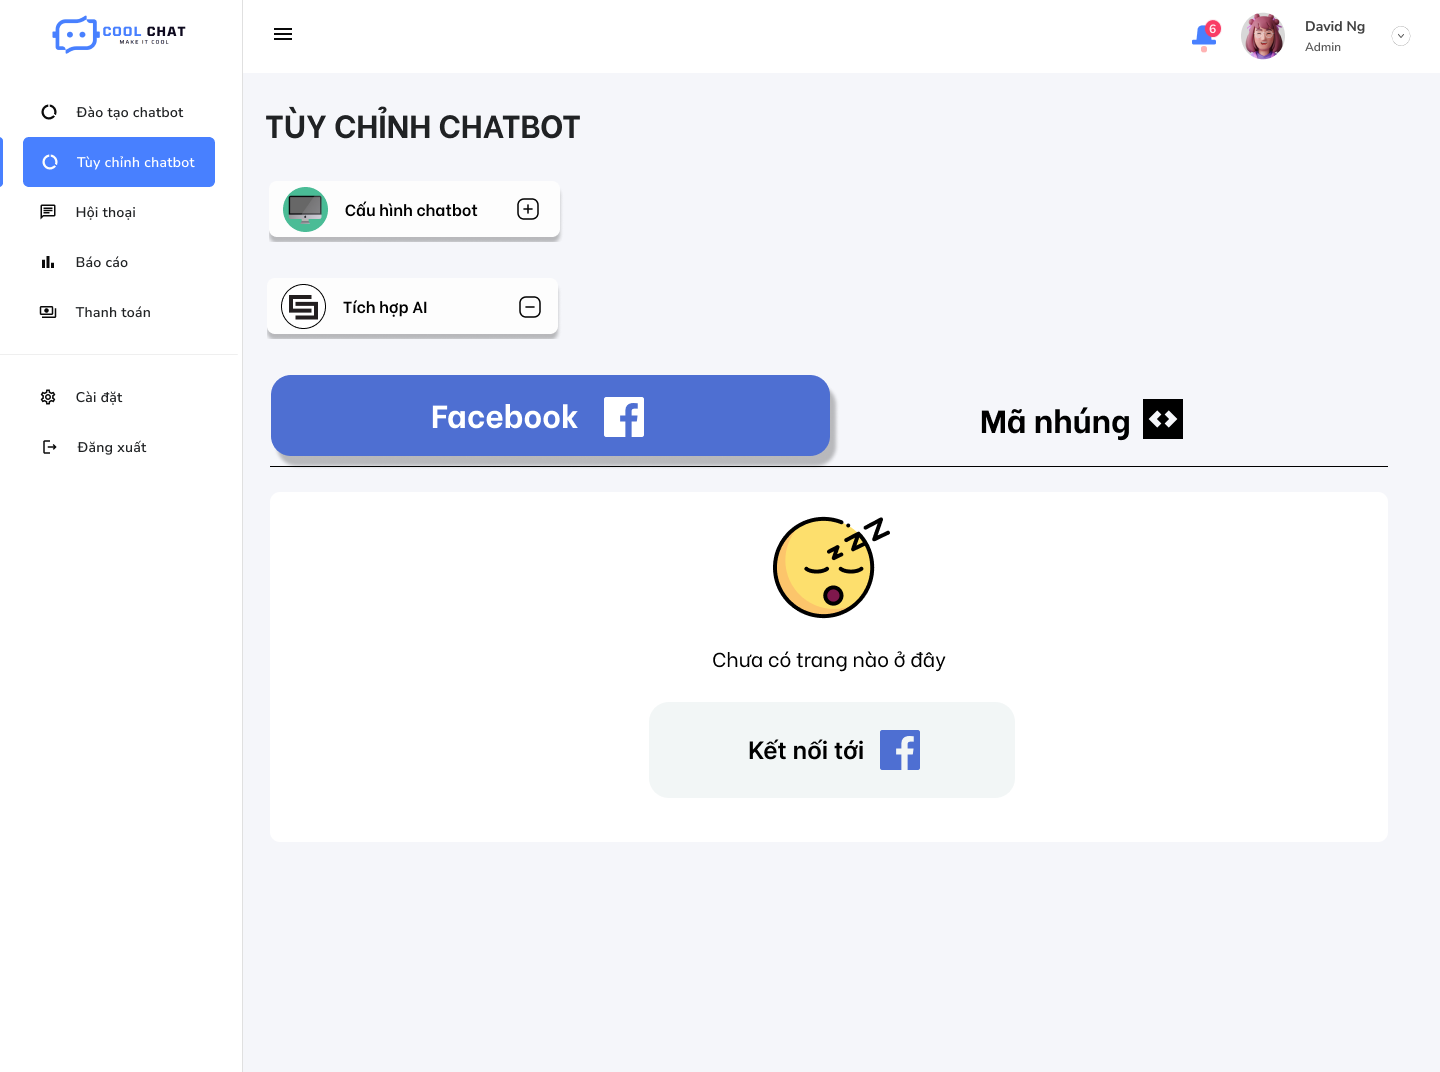
\includegraphics[width=\textwidth]{Figma/THAIFB.png}}
	\vspace{0.5cm}
	\caption{Giao diện Tích hợp qua Facebook}
	\label{fig:enter-label}
\end{figure}

\begin{figure}[H]
	\centering
	\fbox{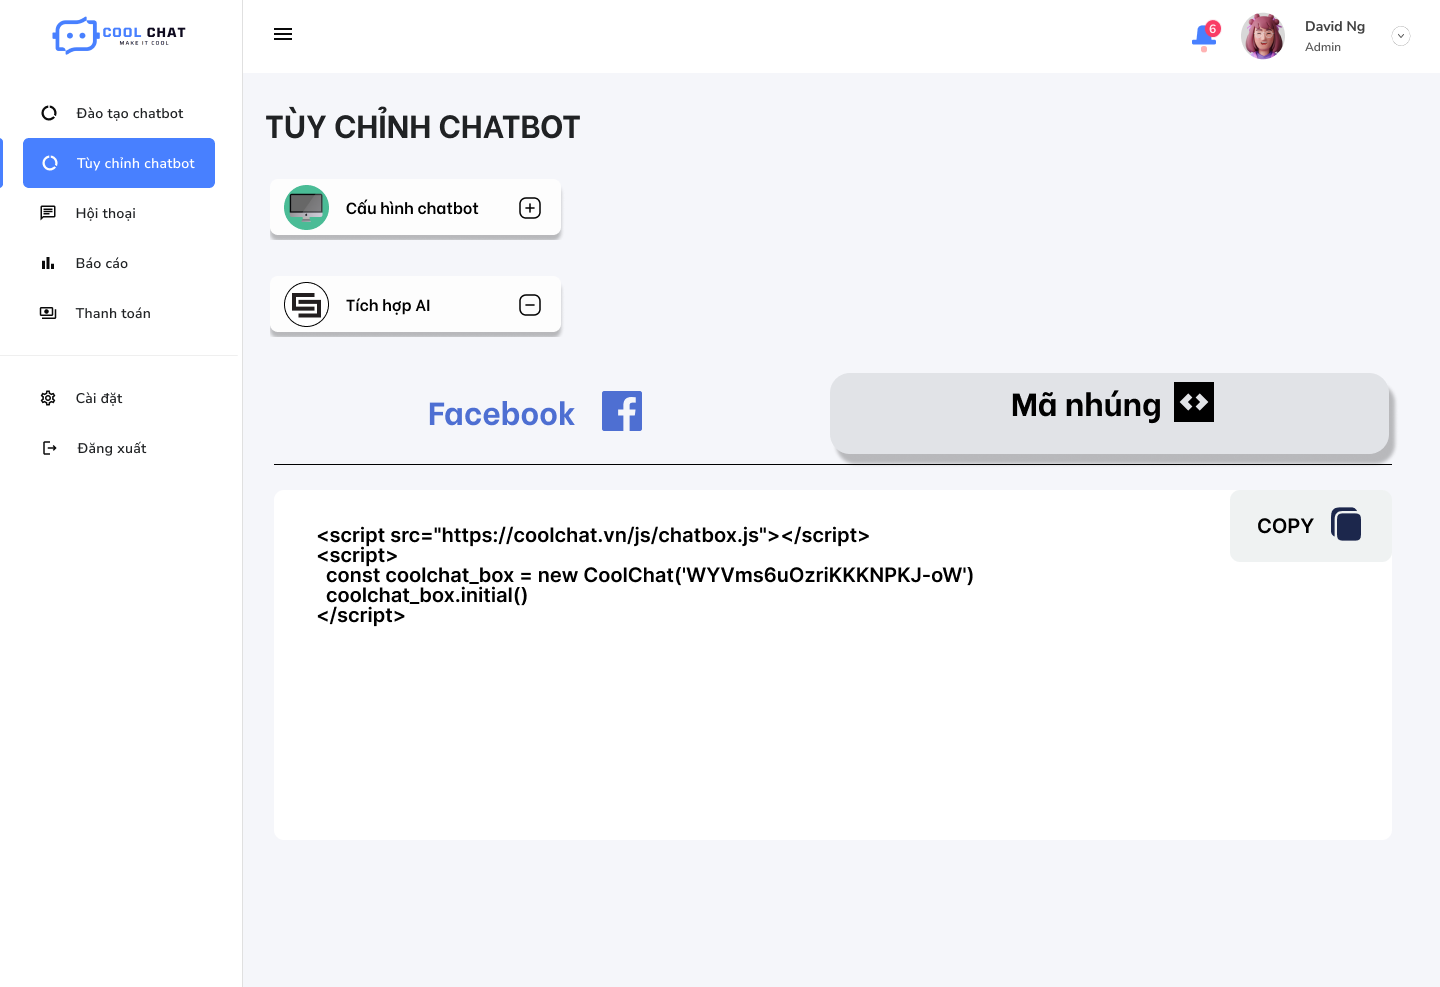
\includegraphics[width=\textwidth]{Figma/THAIMN.png}}
	\vspace{0.5cm}
	\caption{Giao diện Tích hợp qua mã nhúng}
	\label{fig:enter-label}
\end{figure}

\subsubsection{Trang Hội thoại}
\begin{figure}[H]
	\centering
	\fbox{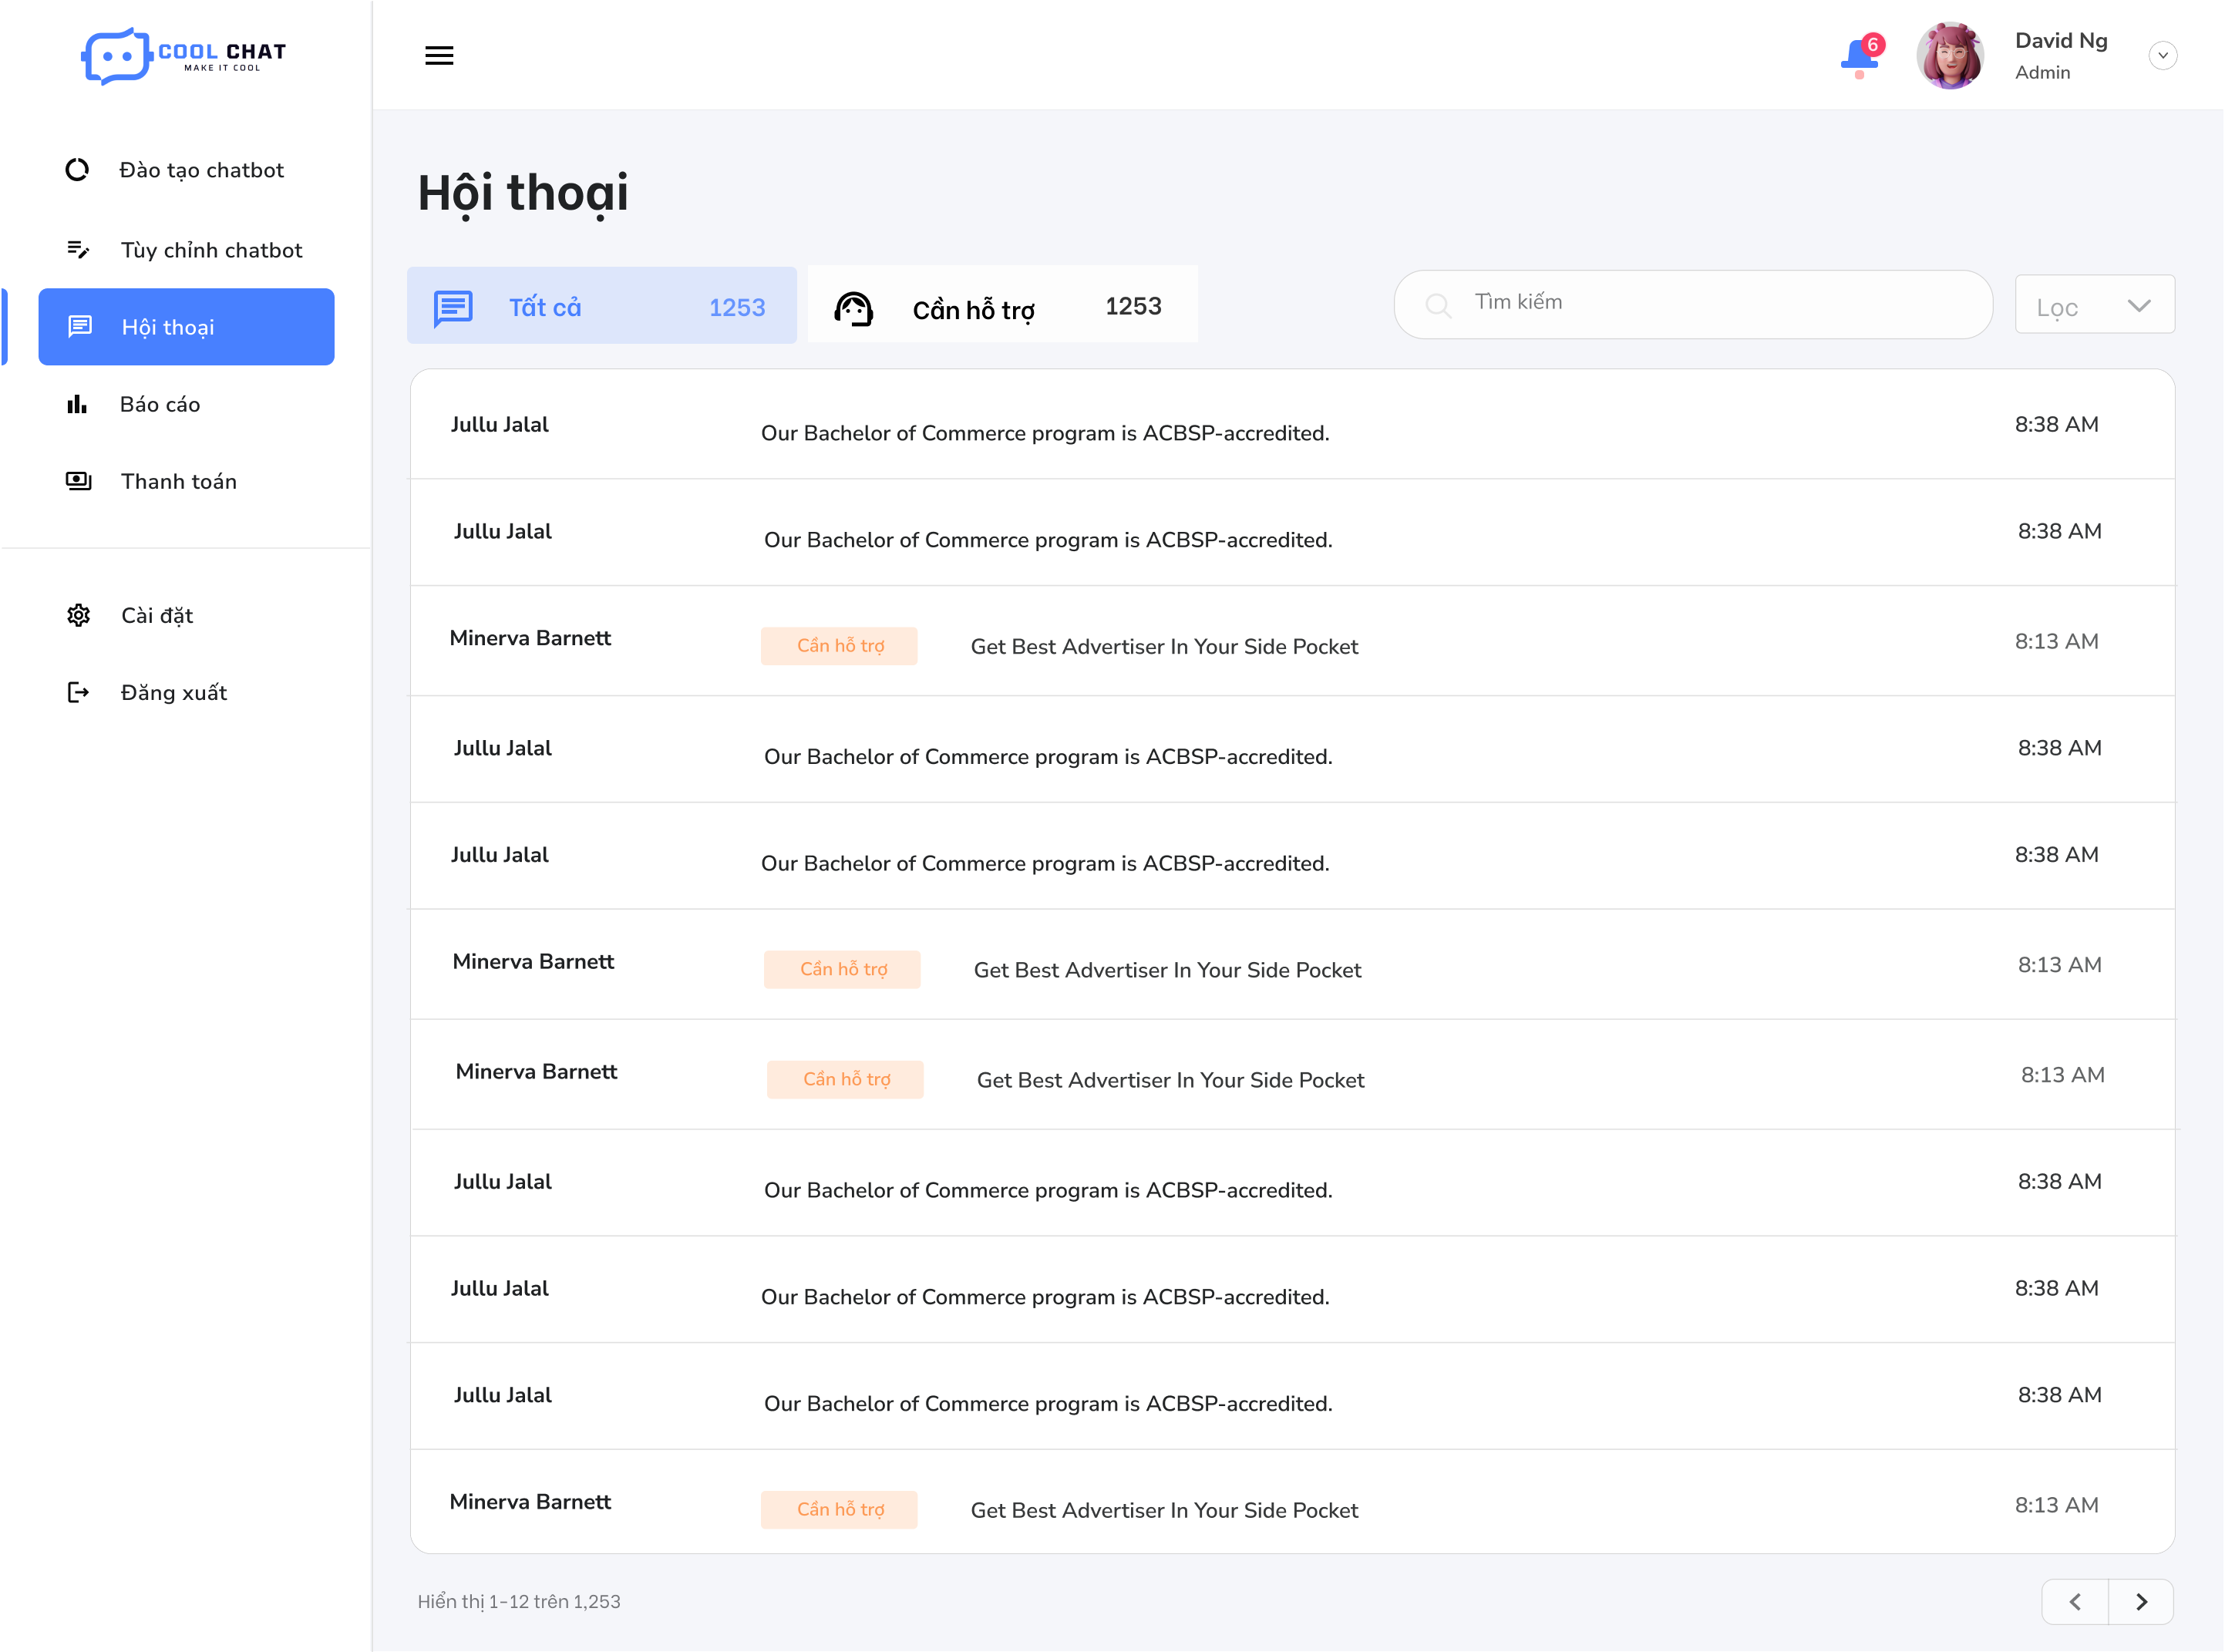
\includegraphics[width=\textwidth]{Figma/chat_1.png}}
	\vspace{0.5cm}
	\caption{Giao diện trang Hội thoại}
	\label{fig:enter-label}
\end{figure}

Giao diện trang Hội thoại để hiển thị danh sách các cuộc hội thoại, giao diện bao gồm theo thứ tự từ trên xuống dưới và trái sang phải:
\begin{itemize}
    \item Một nút để xem tất cả cuộc hội thoại và một nút để xem các cuộc hội thoại được gán nhãn cần hỗ trợ.
    \item Thanh tìm kiếm và nút lọc giúp người dùng đi đến cuộc hội thoại cần tìm một cách nhanh nhất.
    \item Danh sách các cuộc hội thoại, mỗi cuộc hội thoại sẽ hiển thị các thông tin cơ bản như là tên khách hàng, nội dung tin nhắn cuối và thời gian gửi gần nhất.
    \item Thanh dưới bao gồm thông tin số cuộc hội thoại có trên màn hình và thanh phân trang.
\end{itemize}

Khi ấn vào một cuộc hội thoại, màn hình sẽ chuyển đến giao diện chi tiết của cuộc hội thoại đó.
\begin{figure}[H]
	\centering
	\fbox{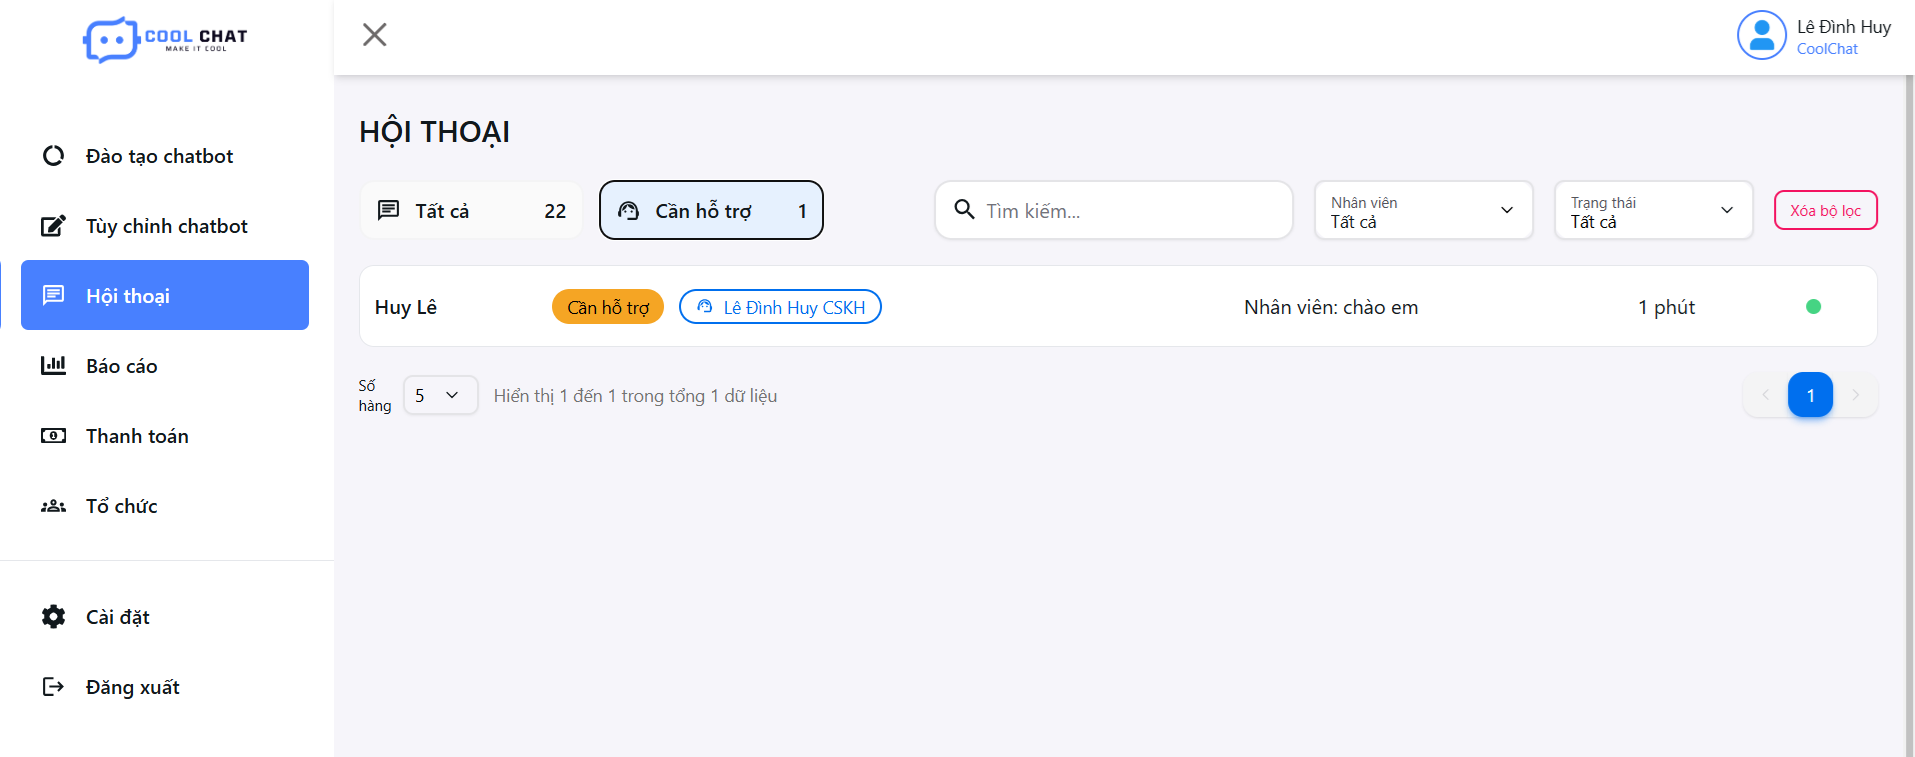
\includegraphics[width=\textwidth]{Figma/chat_2.png}}
	\vspace{0.5cm}
	\caption{Giao diện trang Chi tiết hội thoại}
	\label{fig:enter-label}
\end{figure}

Giao diện gồm có một cửa sổ chat với các tin nhắn hiển thị ở phần trung tâm, mỗi tin nhắn sẽ có nội dung, người gửi và thời gian. Đầu cửa sổ chat gồm có nút quay lại, tên khách hàng, loại hội thoại, nút bật/tắt tính năng tự động chat và nút tùy chọn khác. Đáy cửa sổ chat gồm có nút tải ảnh lên, khung nhập nội dung chat và nút gửi.
\subsubsection{Trang Báo cáo}
\begin{figure}[H]
	\centering
	\fbox{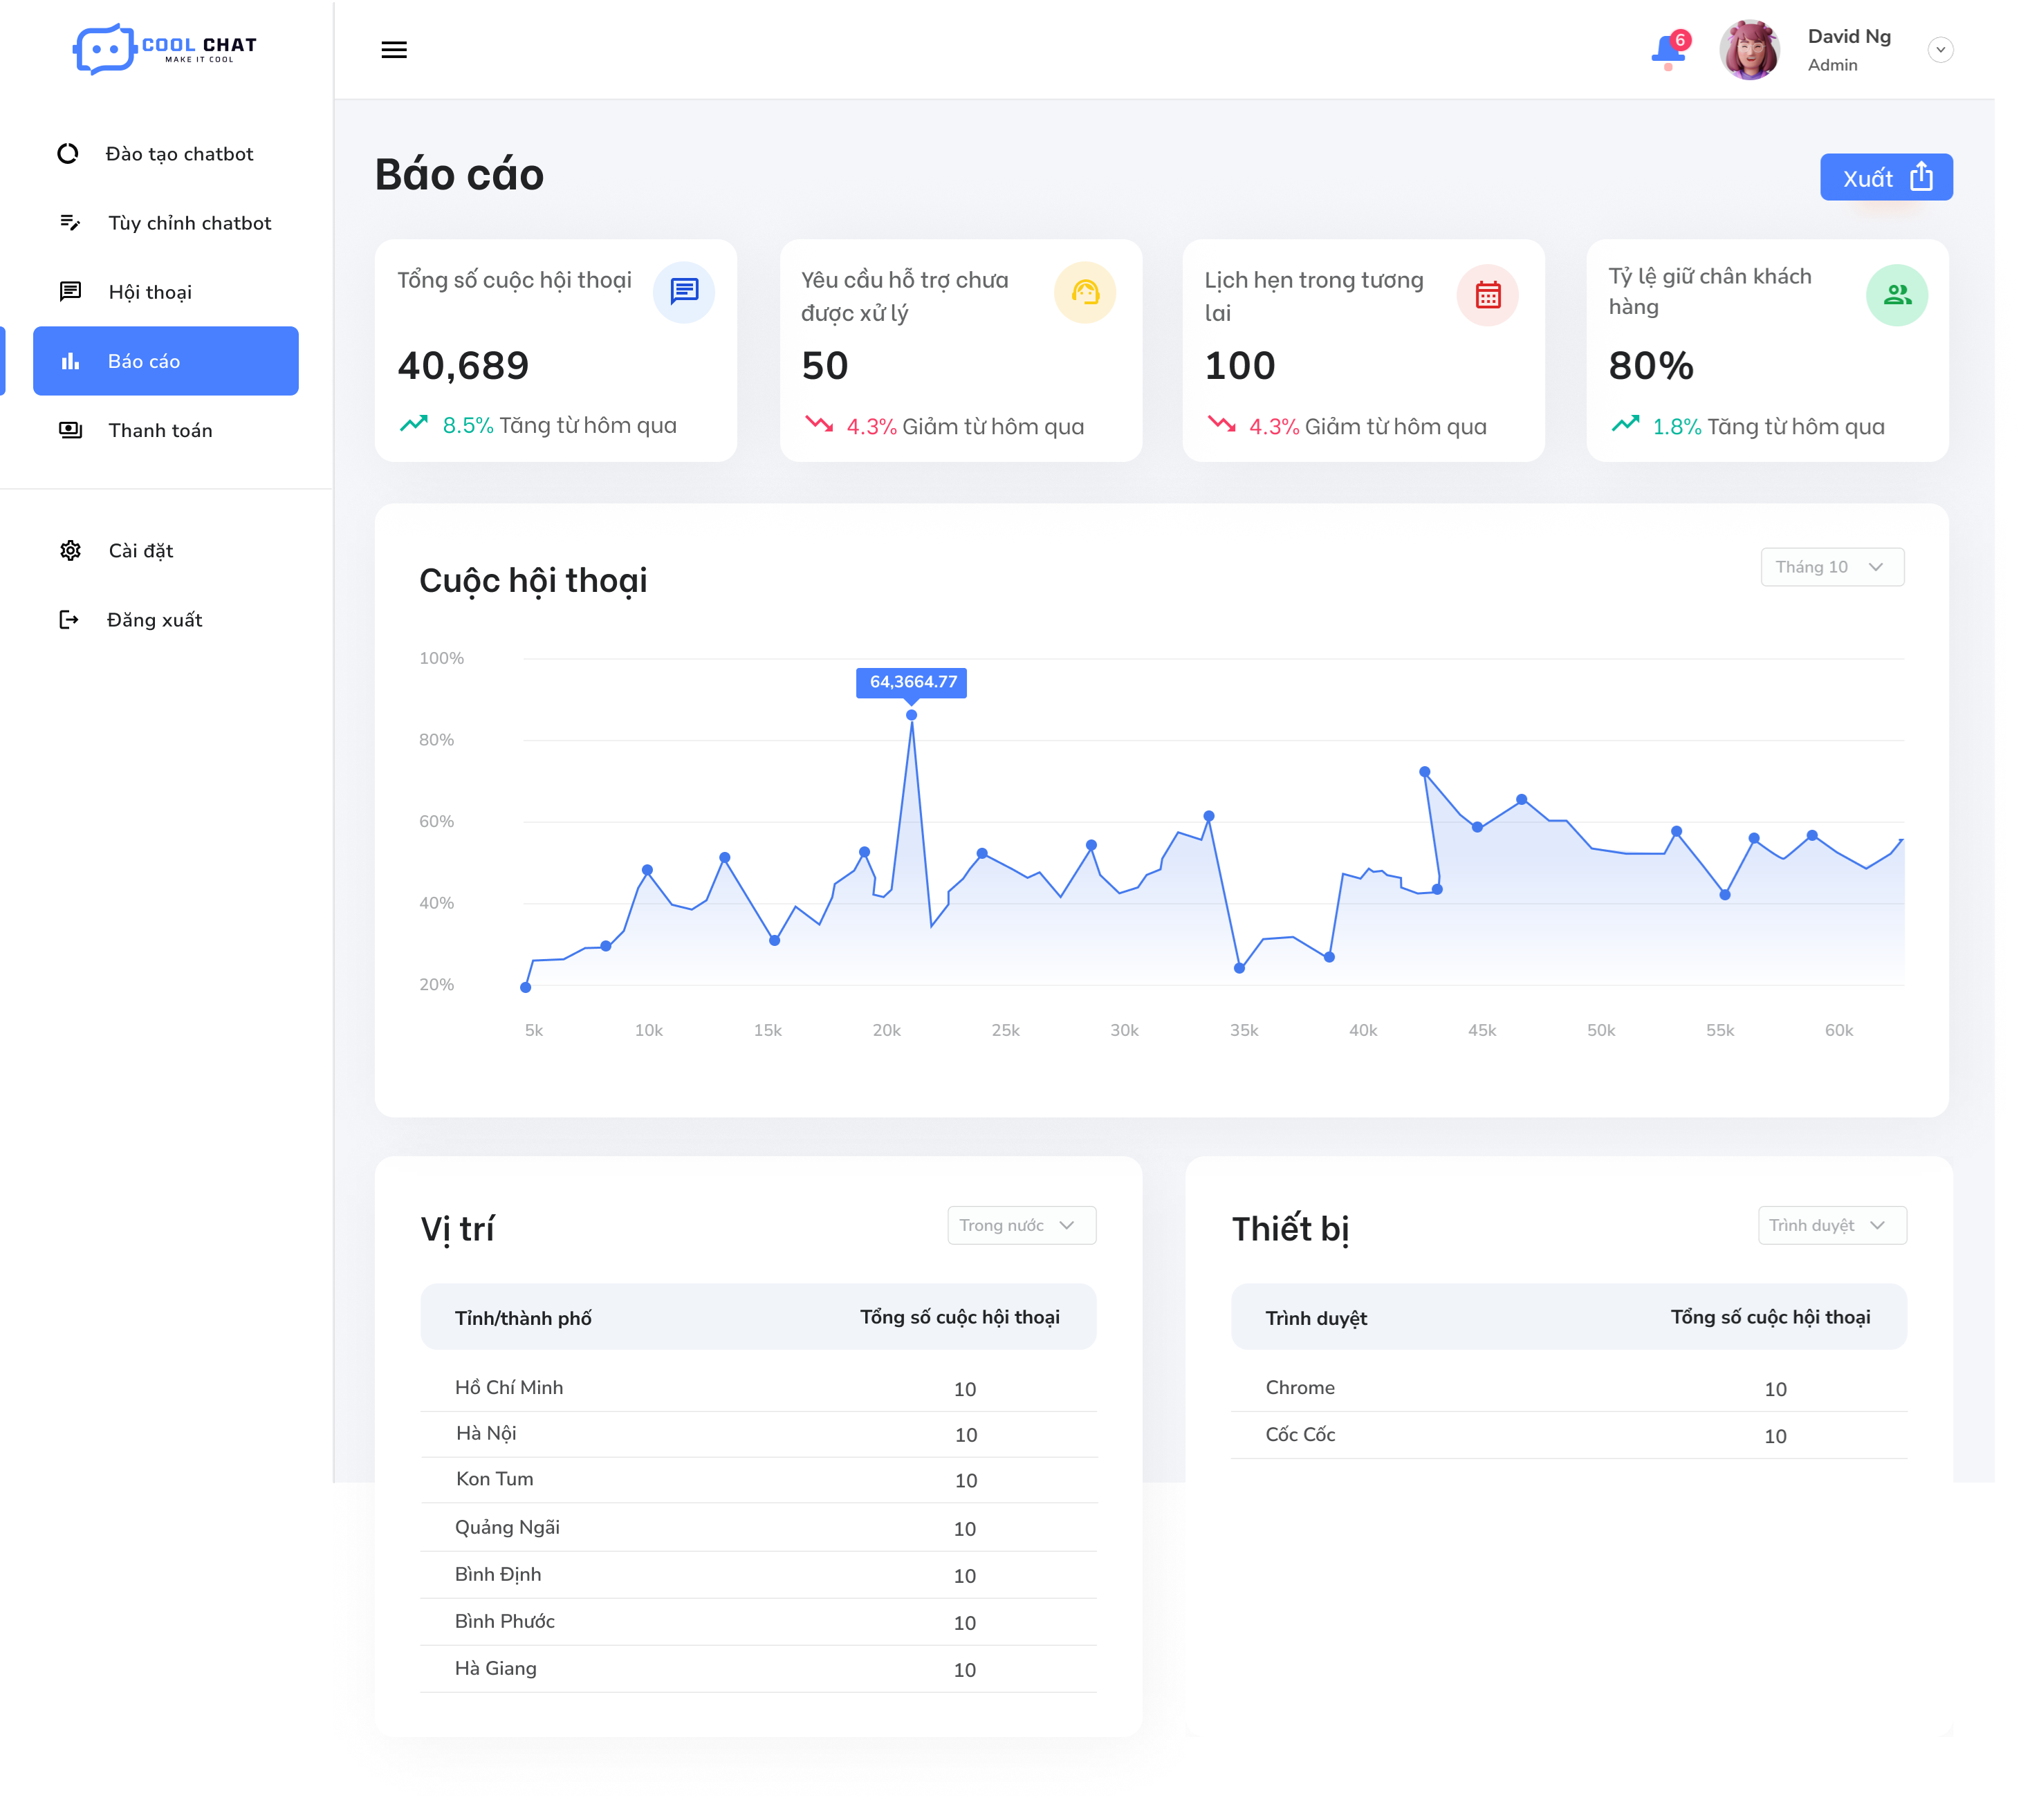
\includegraphics[width=\textwidth]{Figma/report.png}}
	\vspace{0.5cm}
	\caption{Giao diện trang Báo cáo}
	\label{fig:enter-label}
\end{figure}

Giao diện trang Báo cáo để hiển thị một cái nhìn phân tích thông kê về việc sử dụng của chatbot của doanh nghiệp, giao diện gồm có:
\begin{itemize}
	\item Nút xuất dùng để xuất báo cáo ra tệp pdf hoặc xlsx. Khi ấn vào màn hình sẽ hiển lên bản xem trước của báo cáo.
	\item Bên dưới sẽ là thống kê số liệu của 4 số liệu quan trọng bao gồm tổng số cuộc hội thoại, yêu cầu hỗ trợ chưa được xử lý, lịch hẹn trong tương lai, tỷ lệ giữ chân khách hàng. Mỗi số liệu sẽ được biểu thị con số và số phần trăm tăng giảm so với một khoảng thời gian.
	\item Biểu đổ thống kê số cuộc hội thoại theo thời gian.
	\item Bảng số cuộc hội thoại theo vị trí.
	\item Bảng số cuộc hội thoại theo thiết bị.
\end{itemize}
\subsubsection{Trang Thanh toán}
\begin{figure}[H]
	\centering
	\fbox{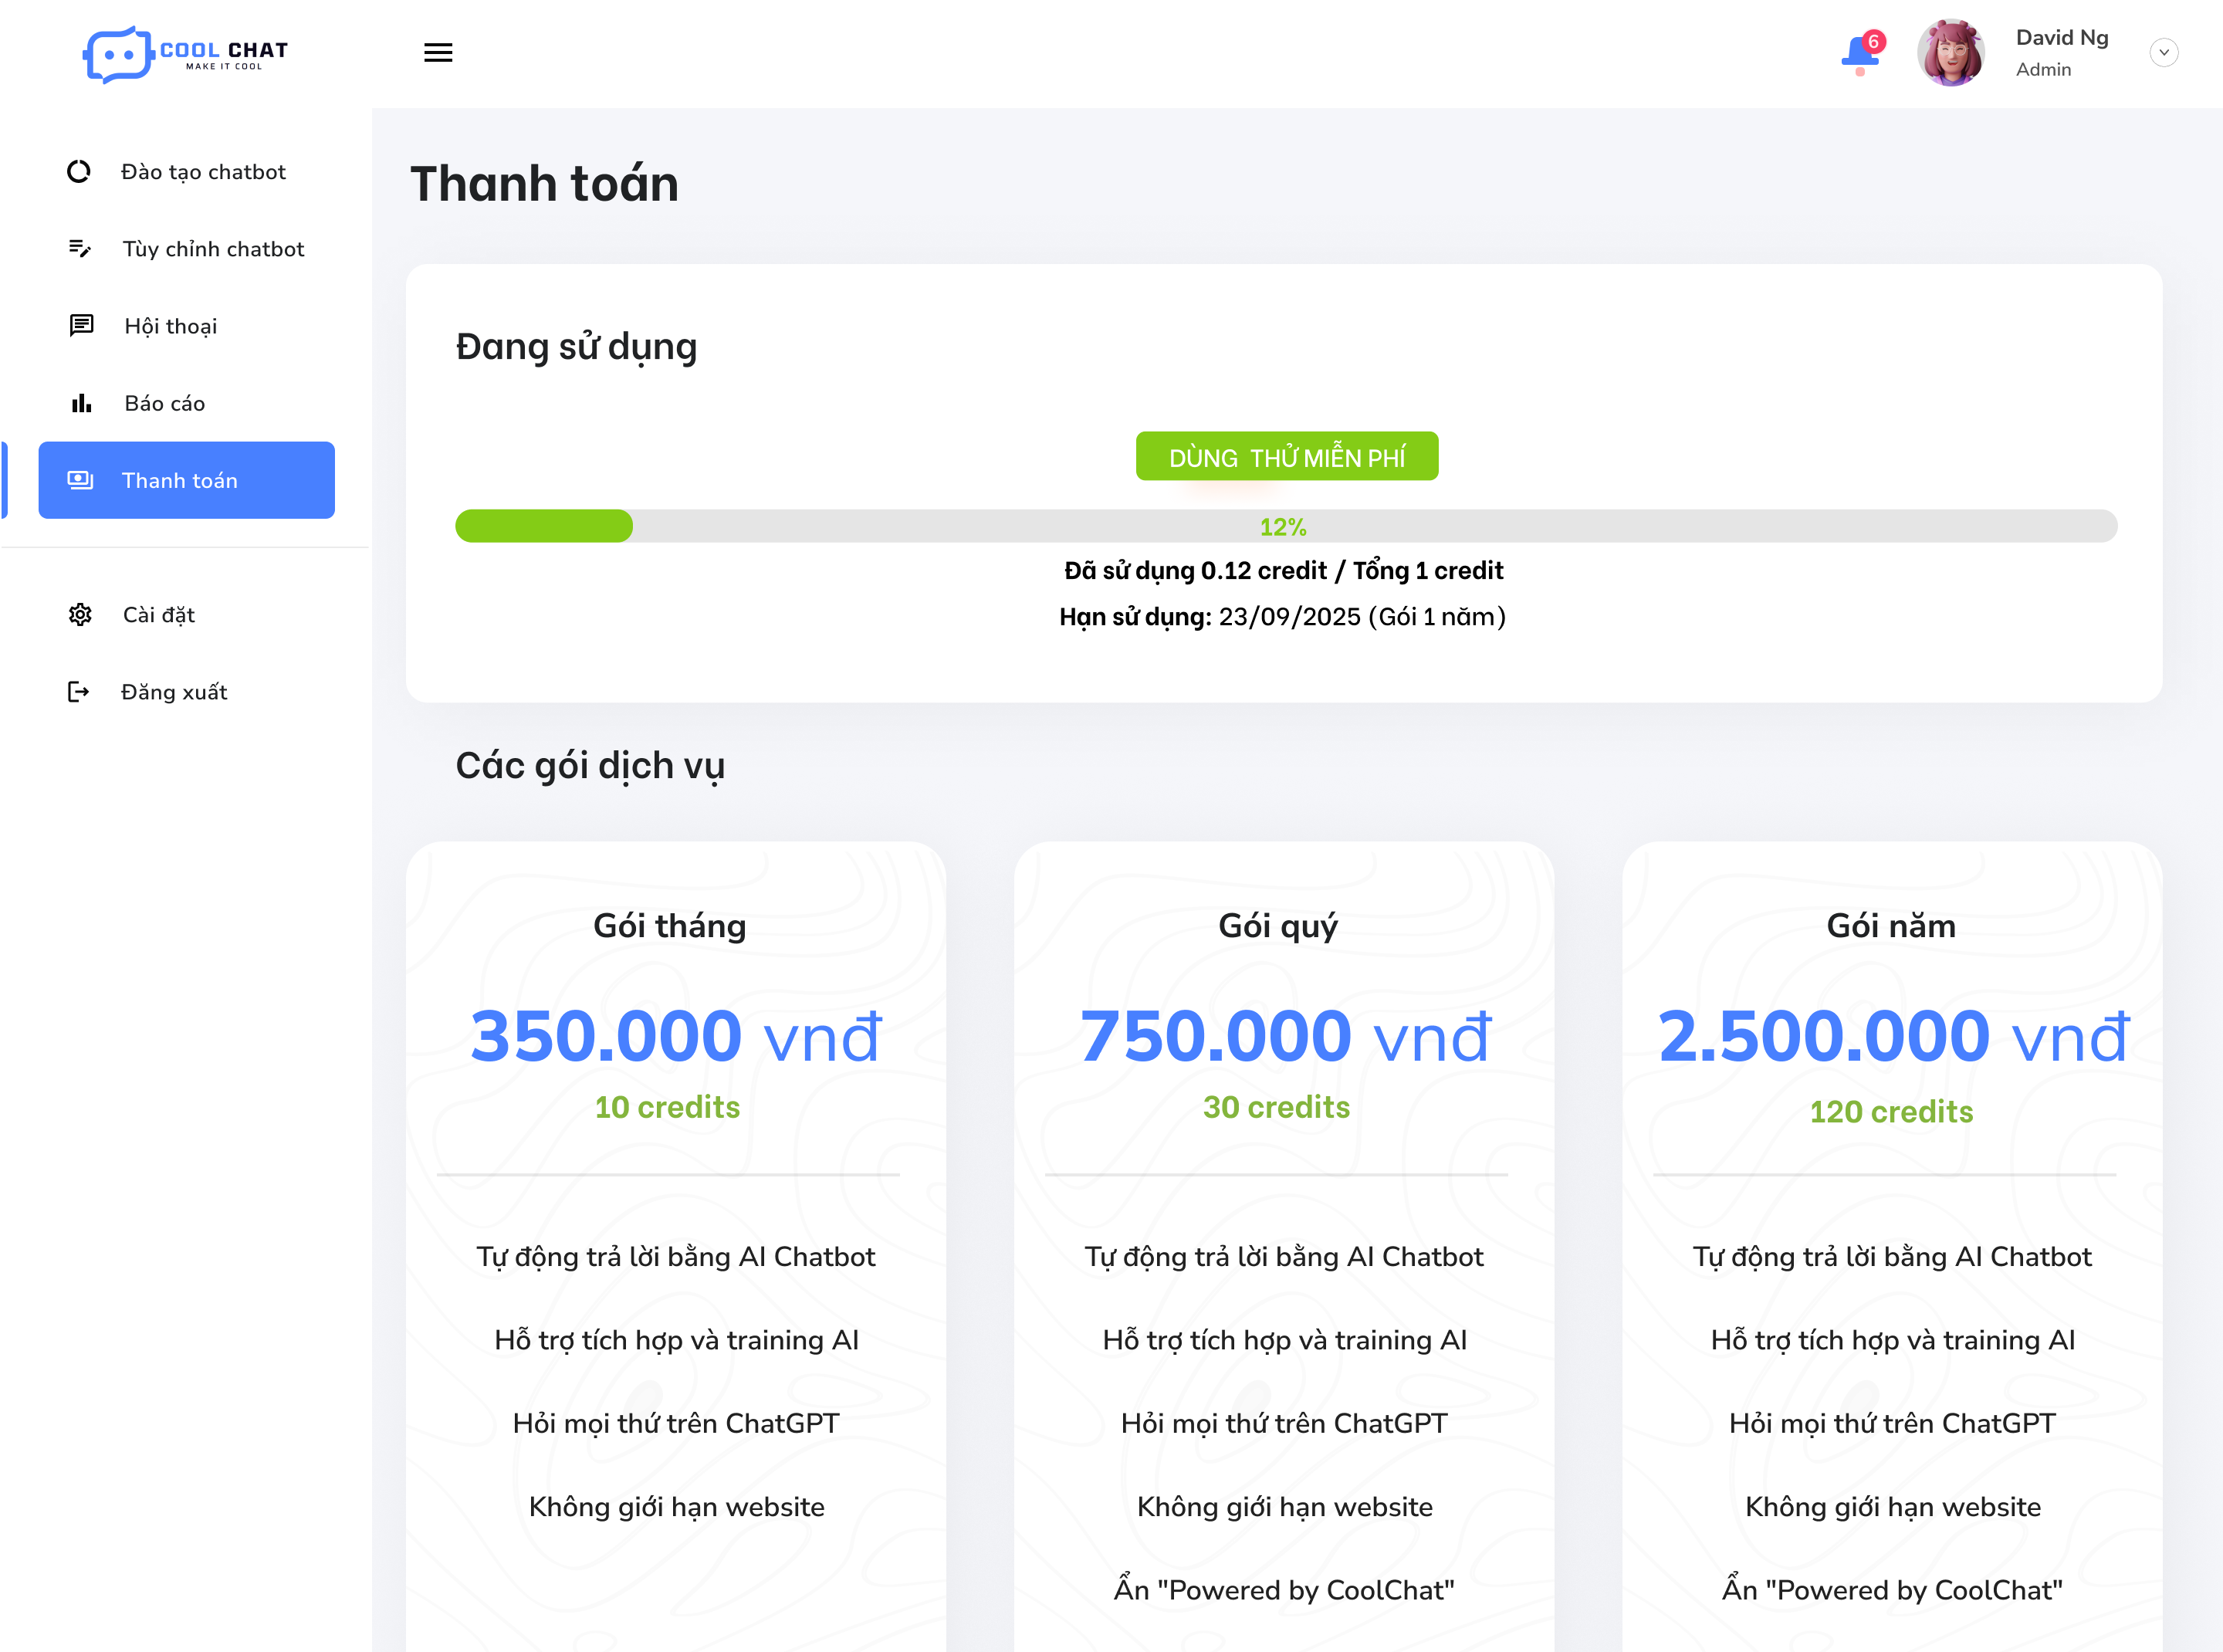
\includegraphics[width=\textwidth]{Figma/subscription.png}}
	\vspace{0.5cm}
	\caption{Giao diện trang Thanh toán}
	\label{fig:enter-label}
\end{figure}

Giao diện trang Thanh toán gồm 2 phần:
\begin{itemize}
	\item Phần Đang sử dụng: biểu thị gói dịch vụ đang sử dụng với số credit tiêu thụ hiện tại được thể hiện trên thanh phần trăm cũng như thời gian của gói.
	\item Biểu phí các gói dịch vụ bao gồm tên gói, giá tiền, số credit, tính năng, nút đăng ký và nút dùng thử.
\end{itemize}
\subsubsection{Trang Cài đặt}
Giao diện này gồm hai tiểu phần: Tài khoản và thông báo - cảnh báo.
\subsubsubsection{Tài khoản}

\begin{figure}[H]
	\centering
	\fbox{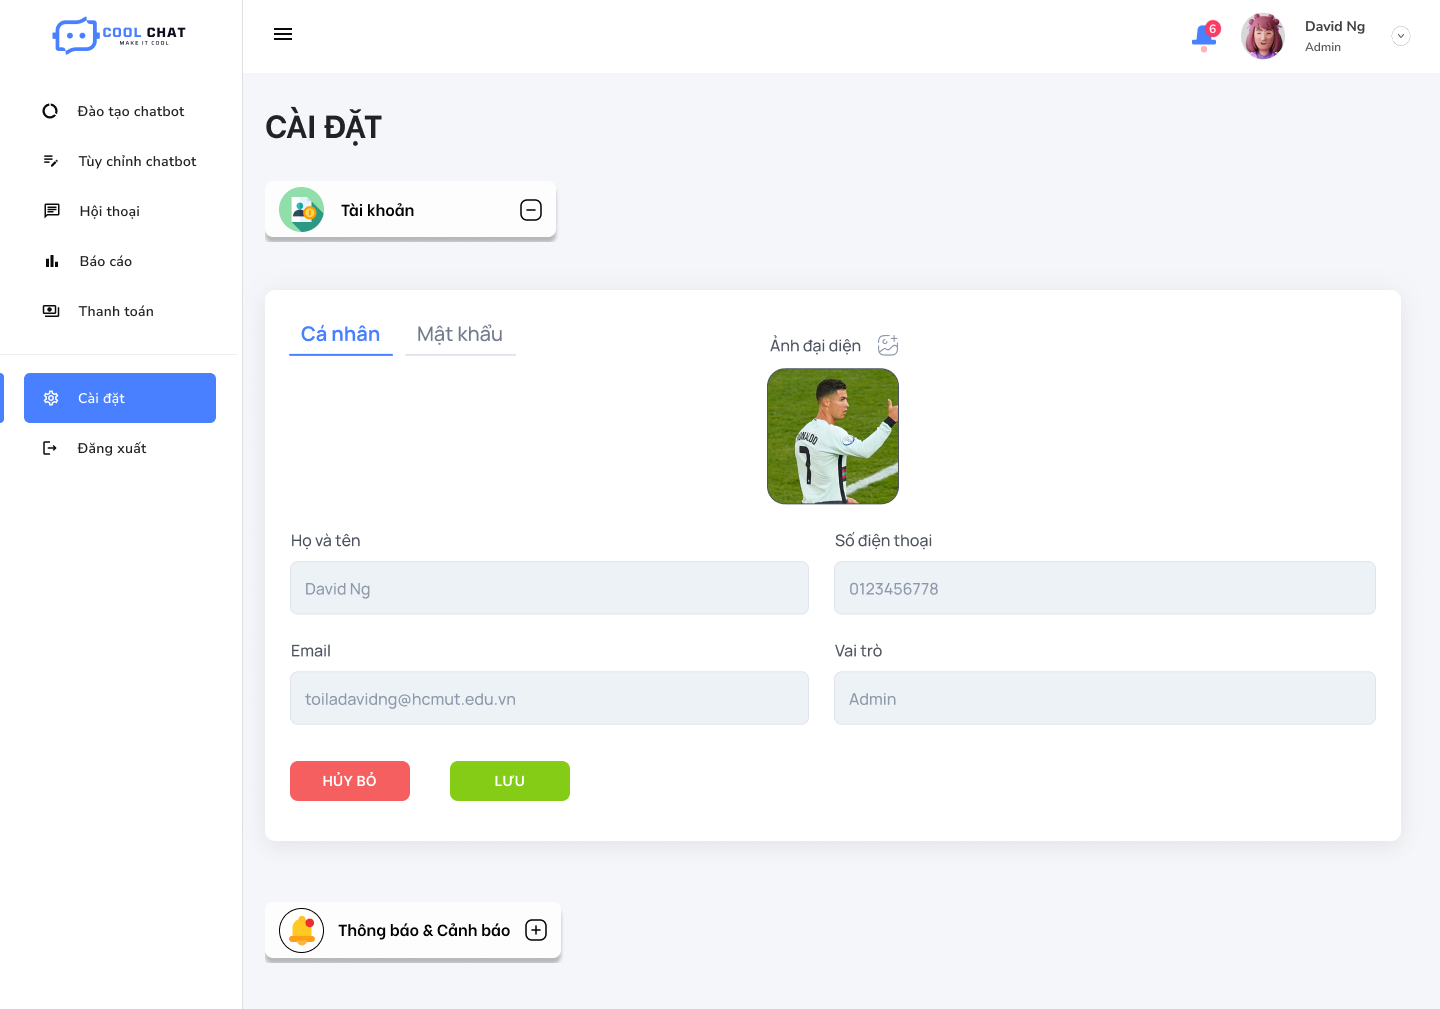
\includegraphics[width=\textwidth]{Figma/CDTK1.png}}
	\vspace{0.5cm}
	\caption{Giao diện trang Tài khoản - Cá nhân}
	\label{fig:enter-label}
\end{figure}

Giao diện Tài khoản cung cấp cho người sử dụng giao diện động linh hoạt chuyển đổi giữa hai loại cài đặt: Cá nhân và Mật khẩu. 
\begin{itemize}
	\item Cá nhân: hiển thị ảnh đại diện, họ và tên, số điện thoại, email và vai trò của người dùng. Email và vai trò là hai thành phần không thể thay đổi.
	
	Người dùng có thể lưu cài đặt (nút đỏ "Hủy bỏ") hoặc ấn "Lưu" (nút màu xanh) để thiết lập thông tin mới.
	\item Mật khẩu: Cho phép người dùng đổi mật khẩu một cách chủ động. Hệ thống yêu cầu nhập cả mật khẩu hiện tại và mật khẩu mới mới có thể thay đổi được mật khẩu.
\end{itemize}
\begin{figure}[H]
	\centering
	\fbox{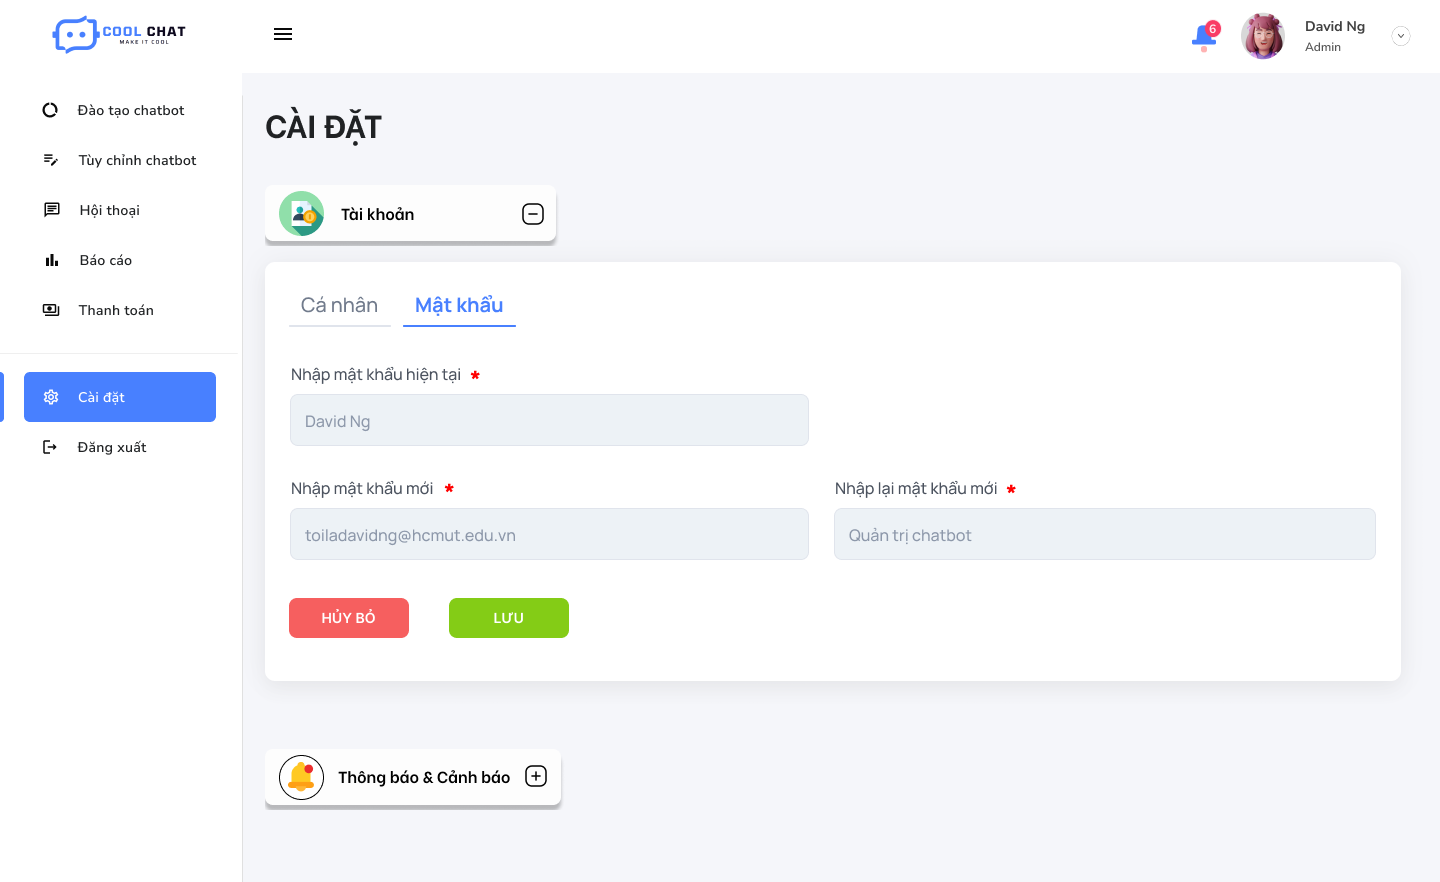
\includegraphics[width=\textwidth]{Figma/CDTK2.png}}
	\vspace{0.5cm}
	\caption{Giao diện trang Tài khoản - Mật khẩu}
	\label{fig:enter-label}
\end{figure}

\subsubsubsection{Thông báo và cảnh báo}
Quản trị viên có quyền lựa chọn cách thức nhận thông báo, cảnh báo trong tab "Chung". Hiện tại có 3 phương thức: 
\begin{itemize}
	\item Email.
	\item Trong chính ứng dụng CoolChat.
	\item SMS (số điện thoại).
\end{itemize}

Các ngưỡng cảnh báo có thể tắt / bật theo mong muốn của quản trị viên, đồng thời quản trị viên thiết lập được ngưỡng của các thông số sau: cảnh báo sử dụng token, bộ nhớ đã dùng, cảnh báo lưu lượng truy cập.
\begin{figure}[H]
	\centering
	\fbox{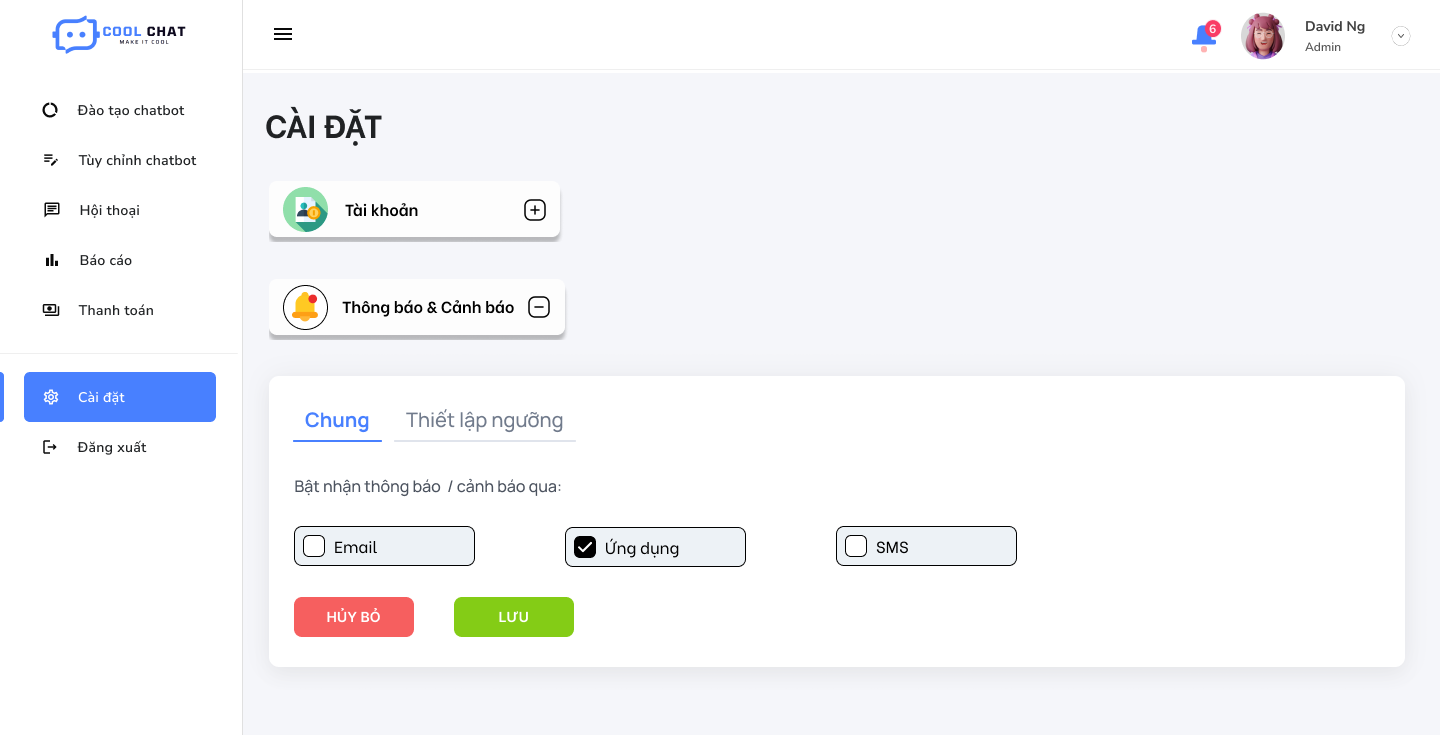
\includegraphics[width=\textwidth]{Figma/TB-CB1.png}}
	\vspace{0.5cm}
	\caption{Giao diện trang Thông báo và cảnh báo - Chung}
	\label{fig:enter-label}
\end{figure}

\begin{figure}[H]
	\centering
	\fbox{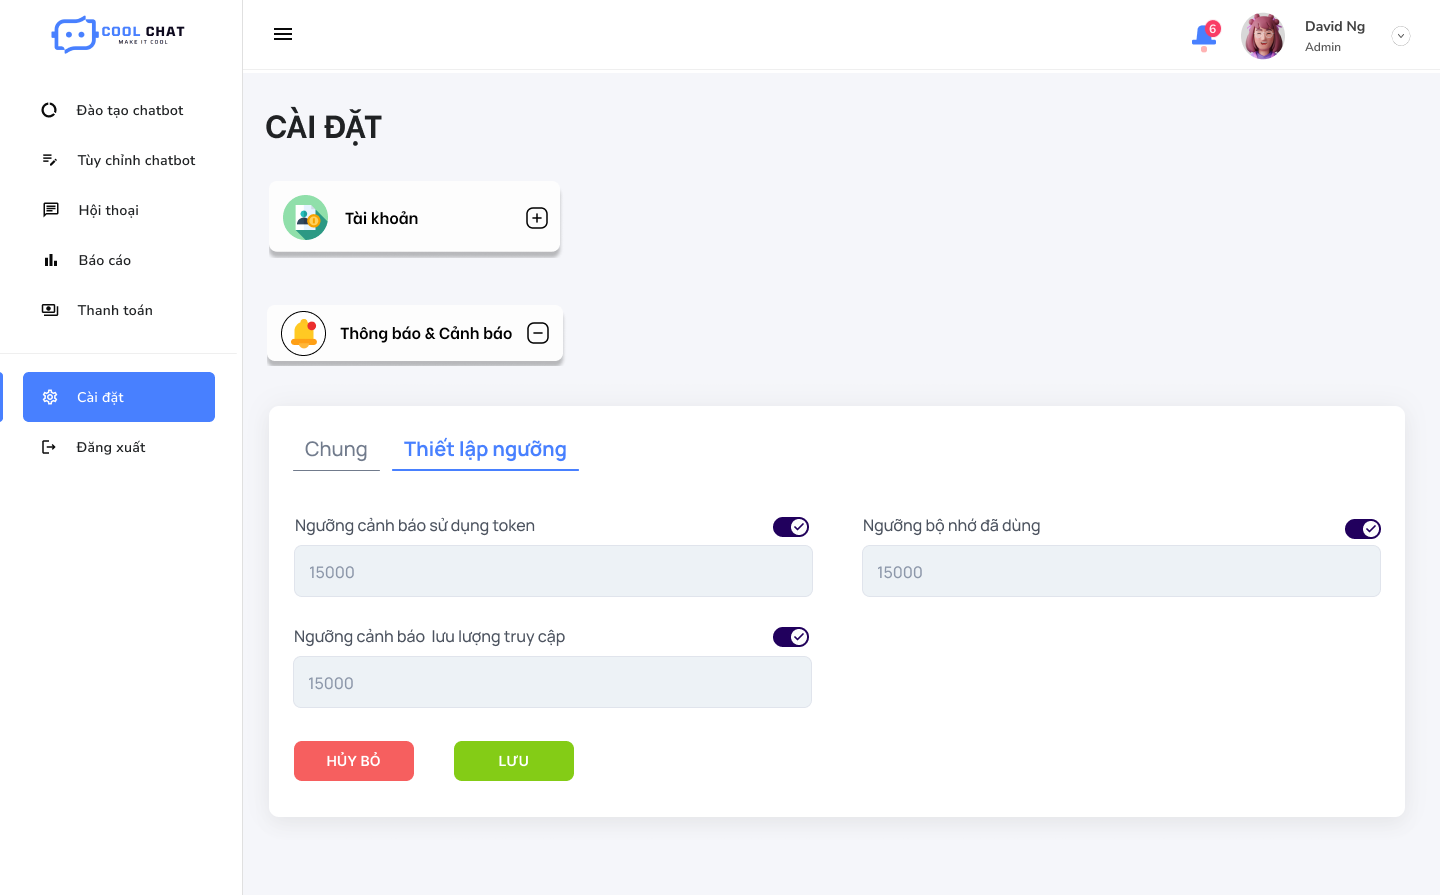
\includegraphics[width=\textwidth]{Figma/TB-CB2.png}}
	\vspace{0.5cm}
	\caption{Giao diện trang Thông báo và cảnh báo - Thiết lập ngưỡng}
	\label{fig:enter-label}
\end{figure}

\subsubsection{Trang Lịch hẹn}
\begin{figure}[H]
	\centering
	\fbox{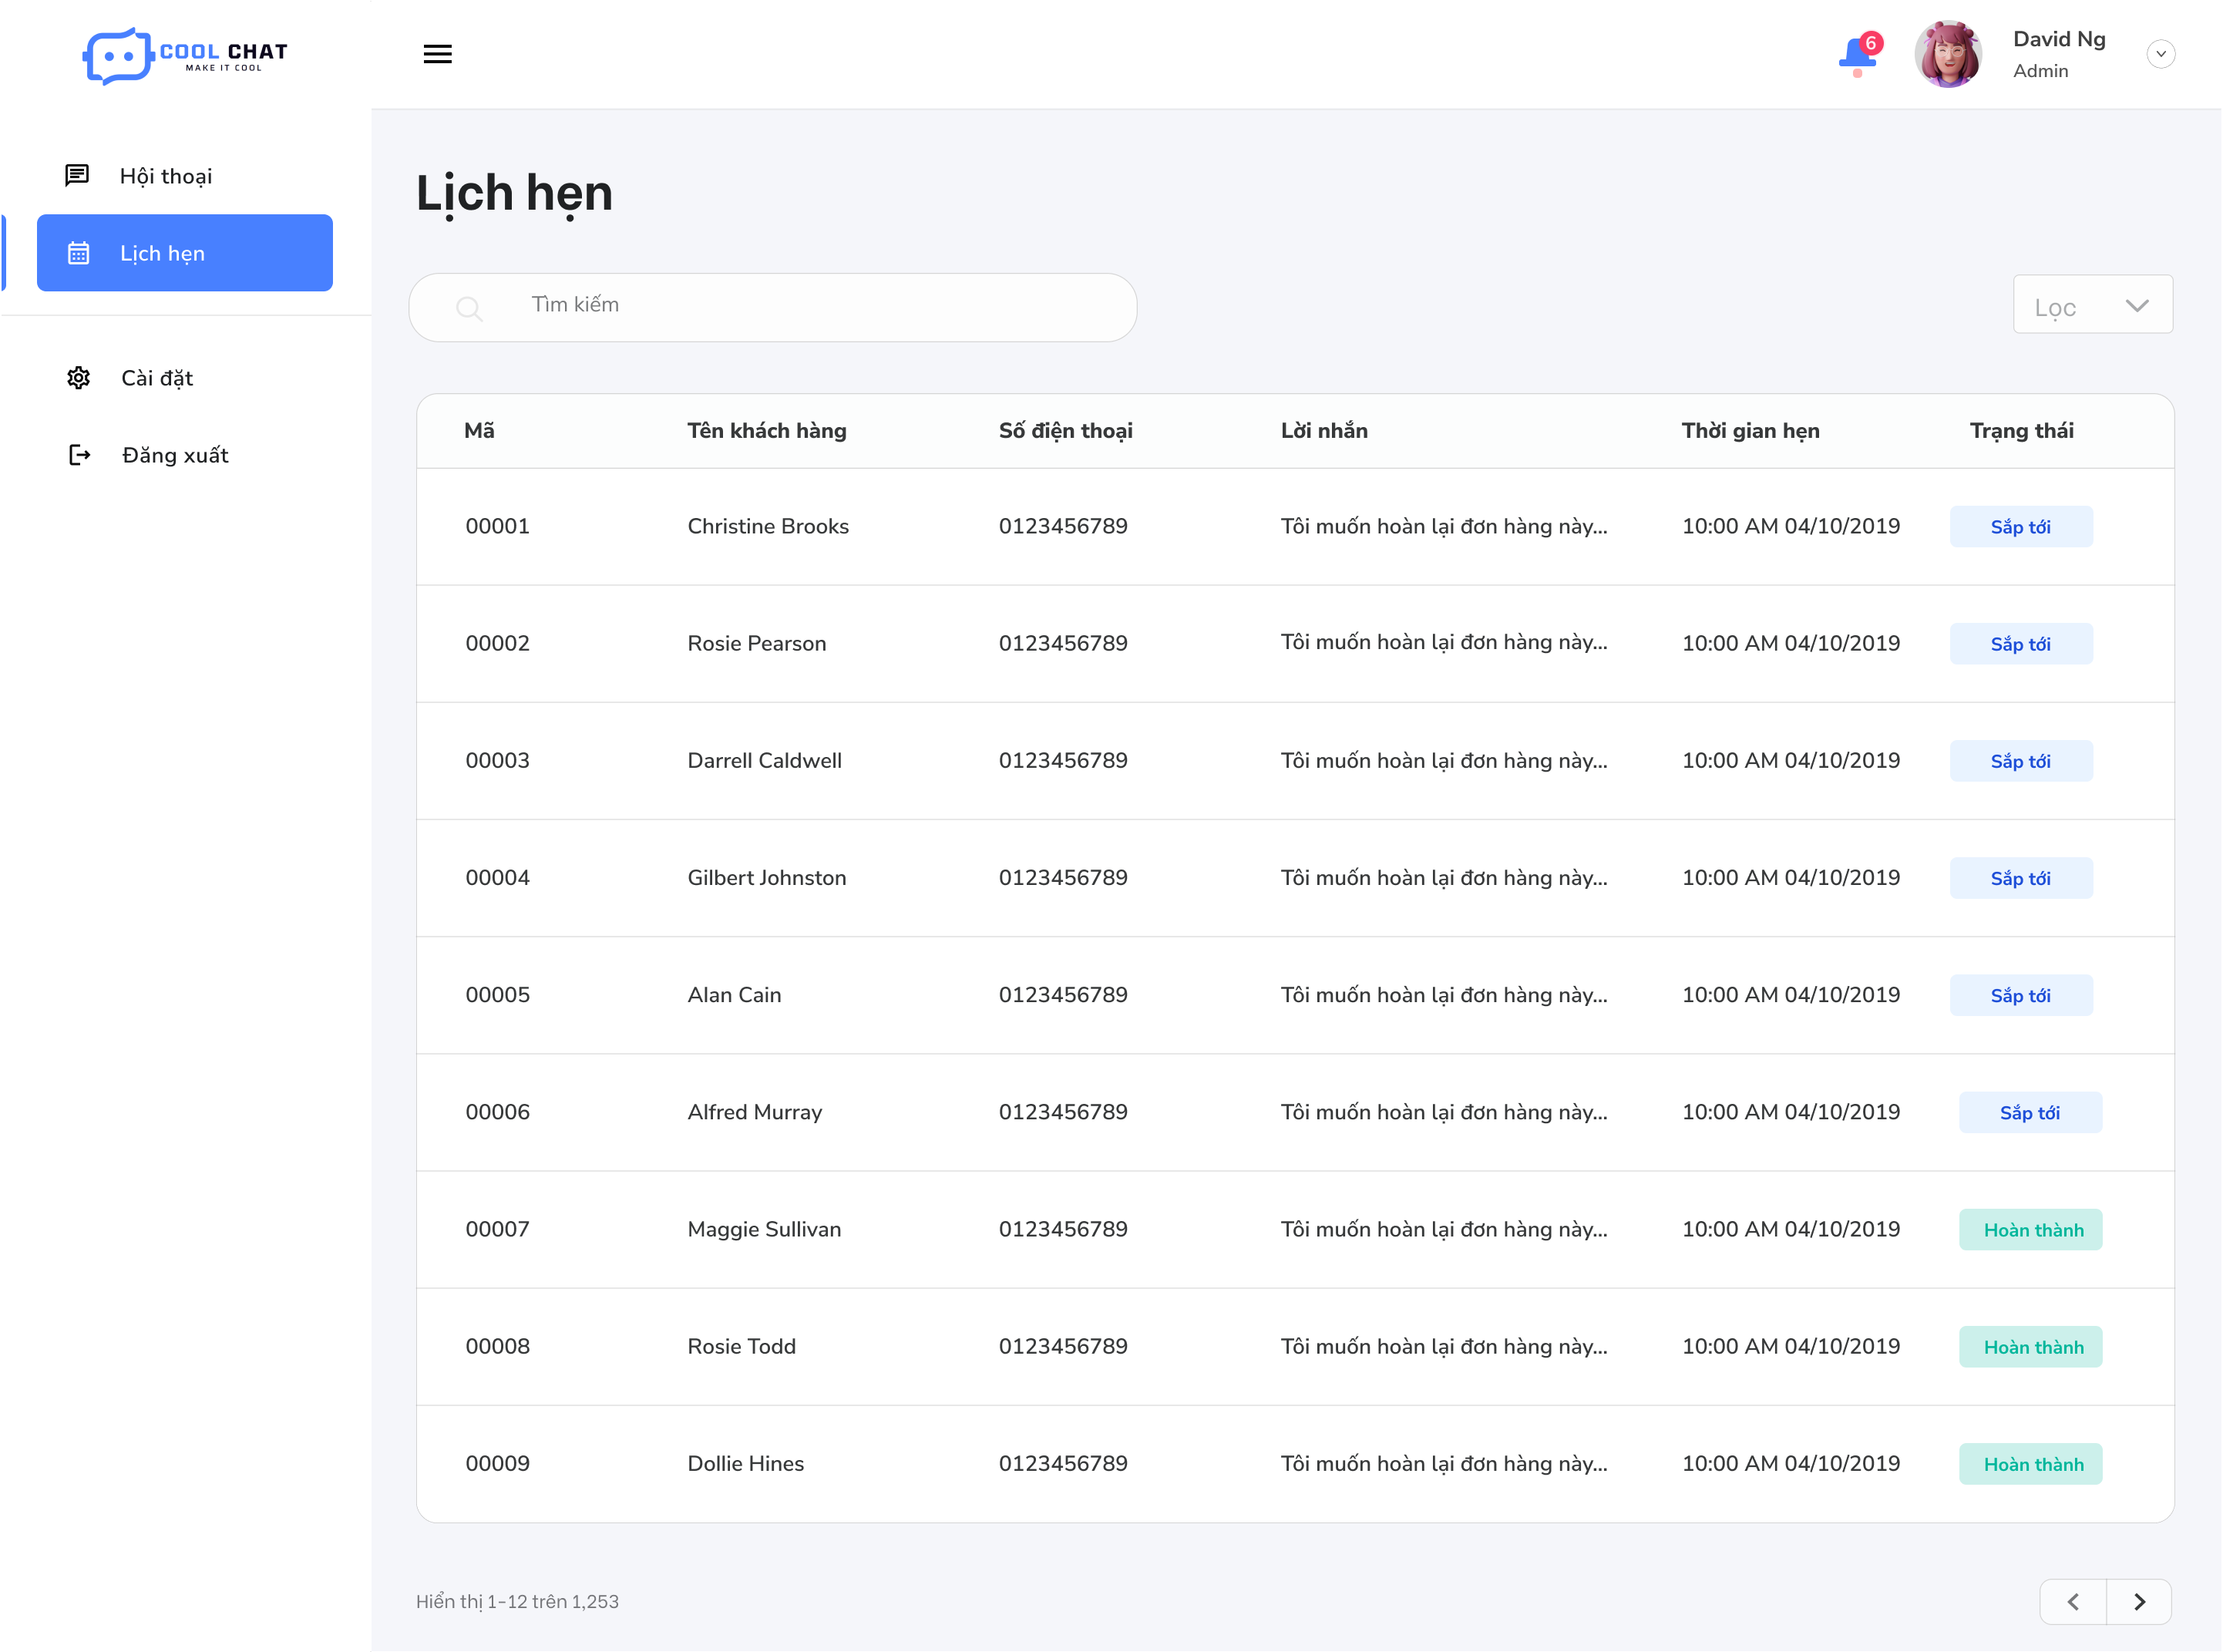
\includegraphics[width=\textwidth]{Figma/appointment.png}}
	\vspace{0.5cm}
	\caption{Giao diện trang Lịch hẹn}
	\label{fig:enter-label}
\end{figure}

Giao diện Lịch hẹn giúp nhân viên CSKH quản lý được các lịch hẹn, giao diện gồm có một thanh tìm kiếm, một nút lọc dữ liệu và một bảng danh sách các lịch hẹn với các trường mã, tên, số điện thoại, lời nhắn, thời gian hẹn và trạng thái, cùng với bên dưới là thanh phân trang cho bảng dữ liệu.

\begin{figure}[H]
	\centering
	\fbox{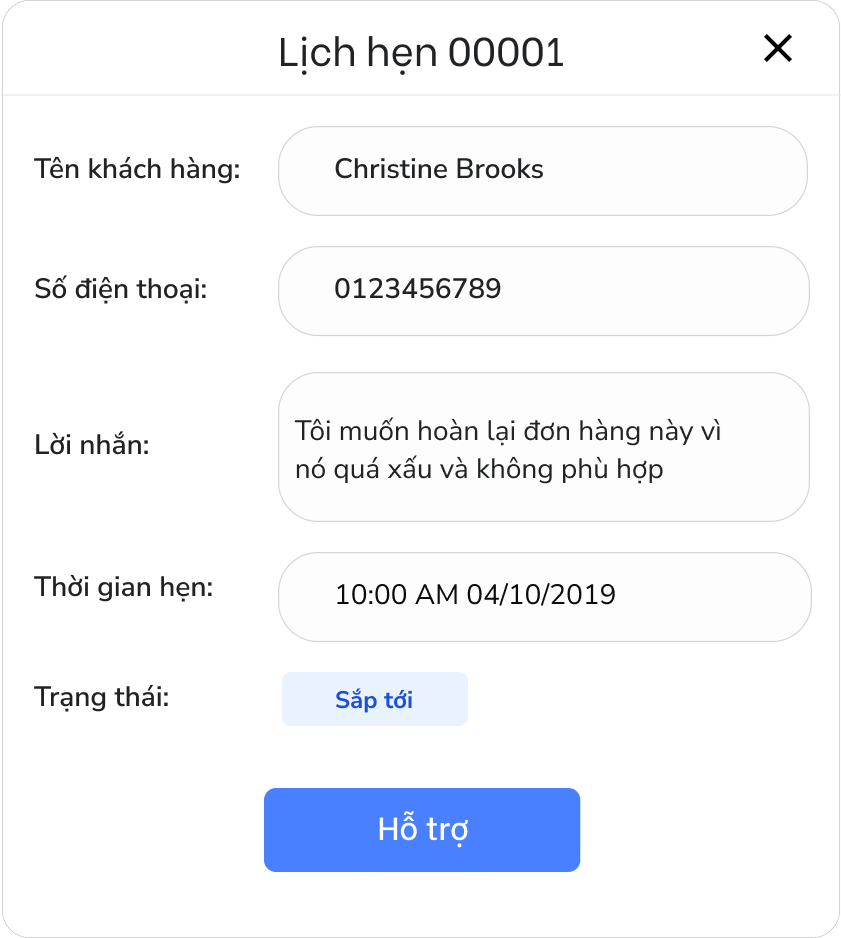
\includegraphics[width=0.5\linewidth]{Figma/lich_hen_detail.png}}
	\vspace{0.5cm}
	\caption{Giao diện trang Lịch hẹn chi tiết}
	\label{fig:enter-label}
\end{figure}

Khi ấn vào một lịch hẹn, ta có thể xem các thông tin chi tiết của lịch hẹn đó. Trong popup chi tiết, sẽ có nút Hỗ trợ để điều hướng người dùng đến đoạn chat.

\subsubsection{Giao diện phía khách hàng}
\begin{figure}[H]
	\centering
	\fbox{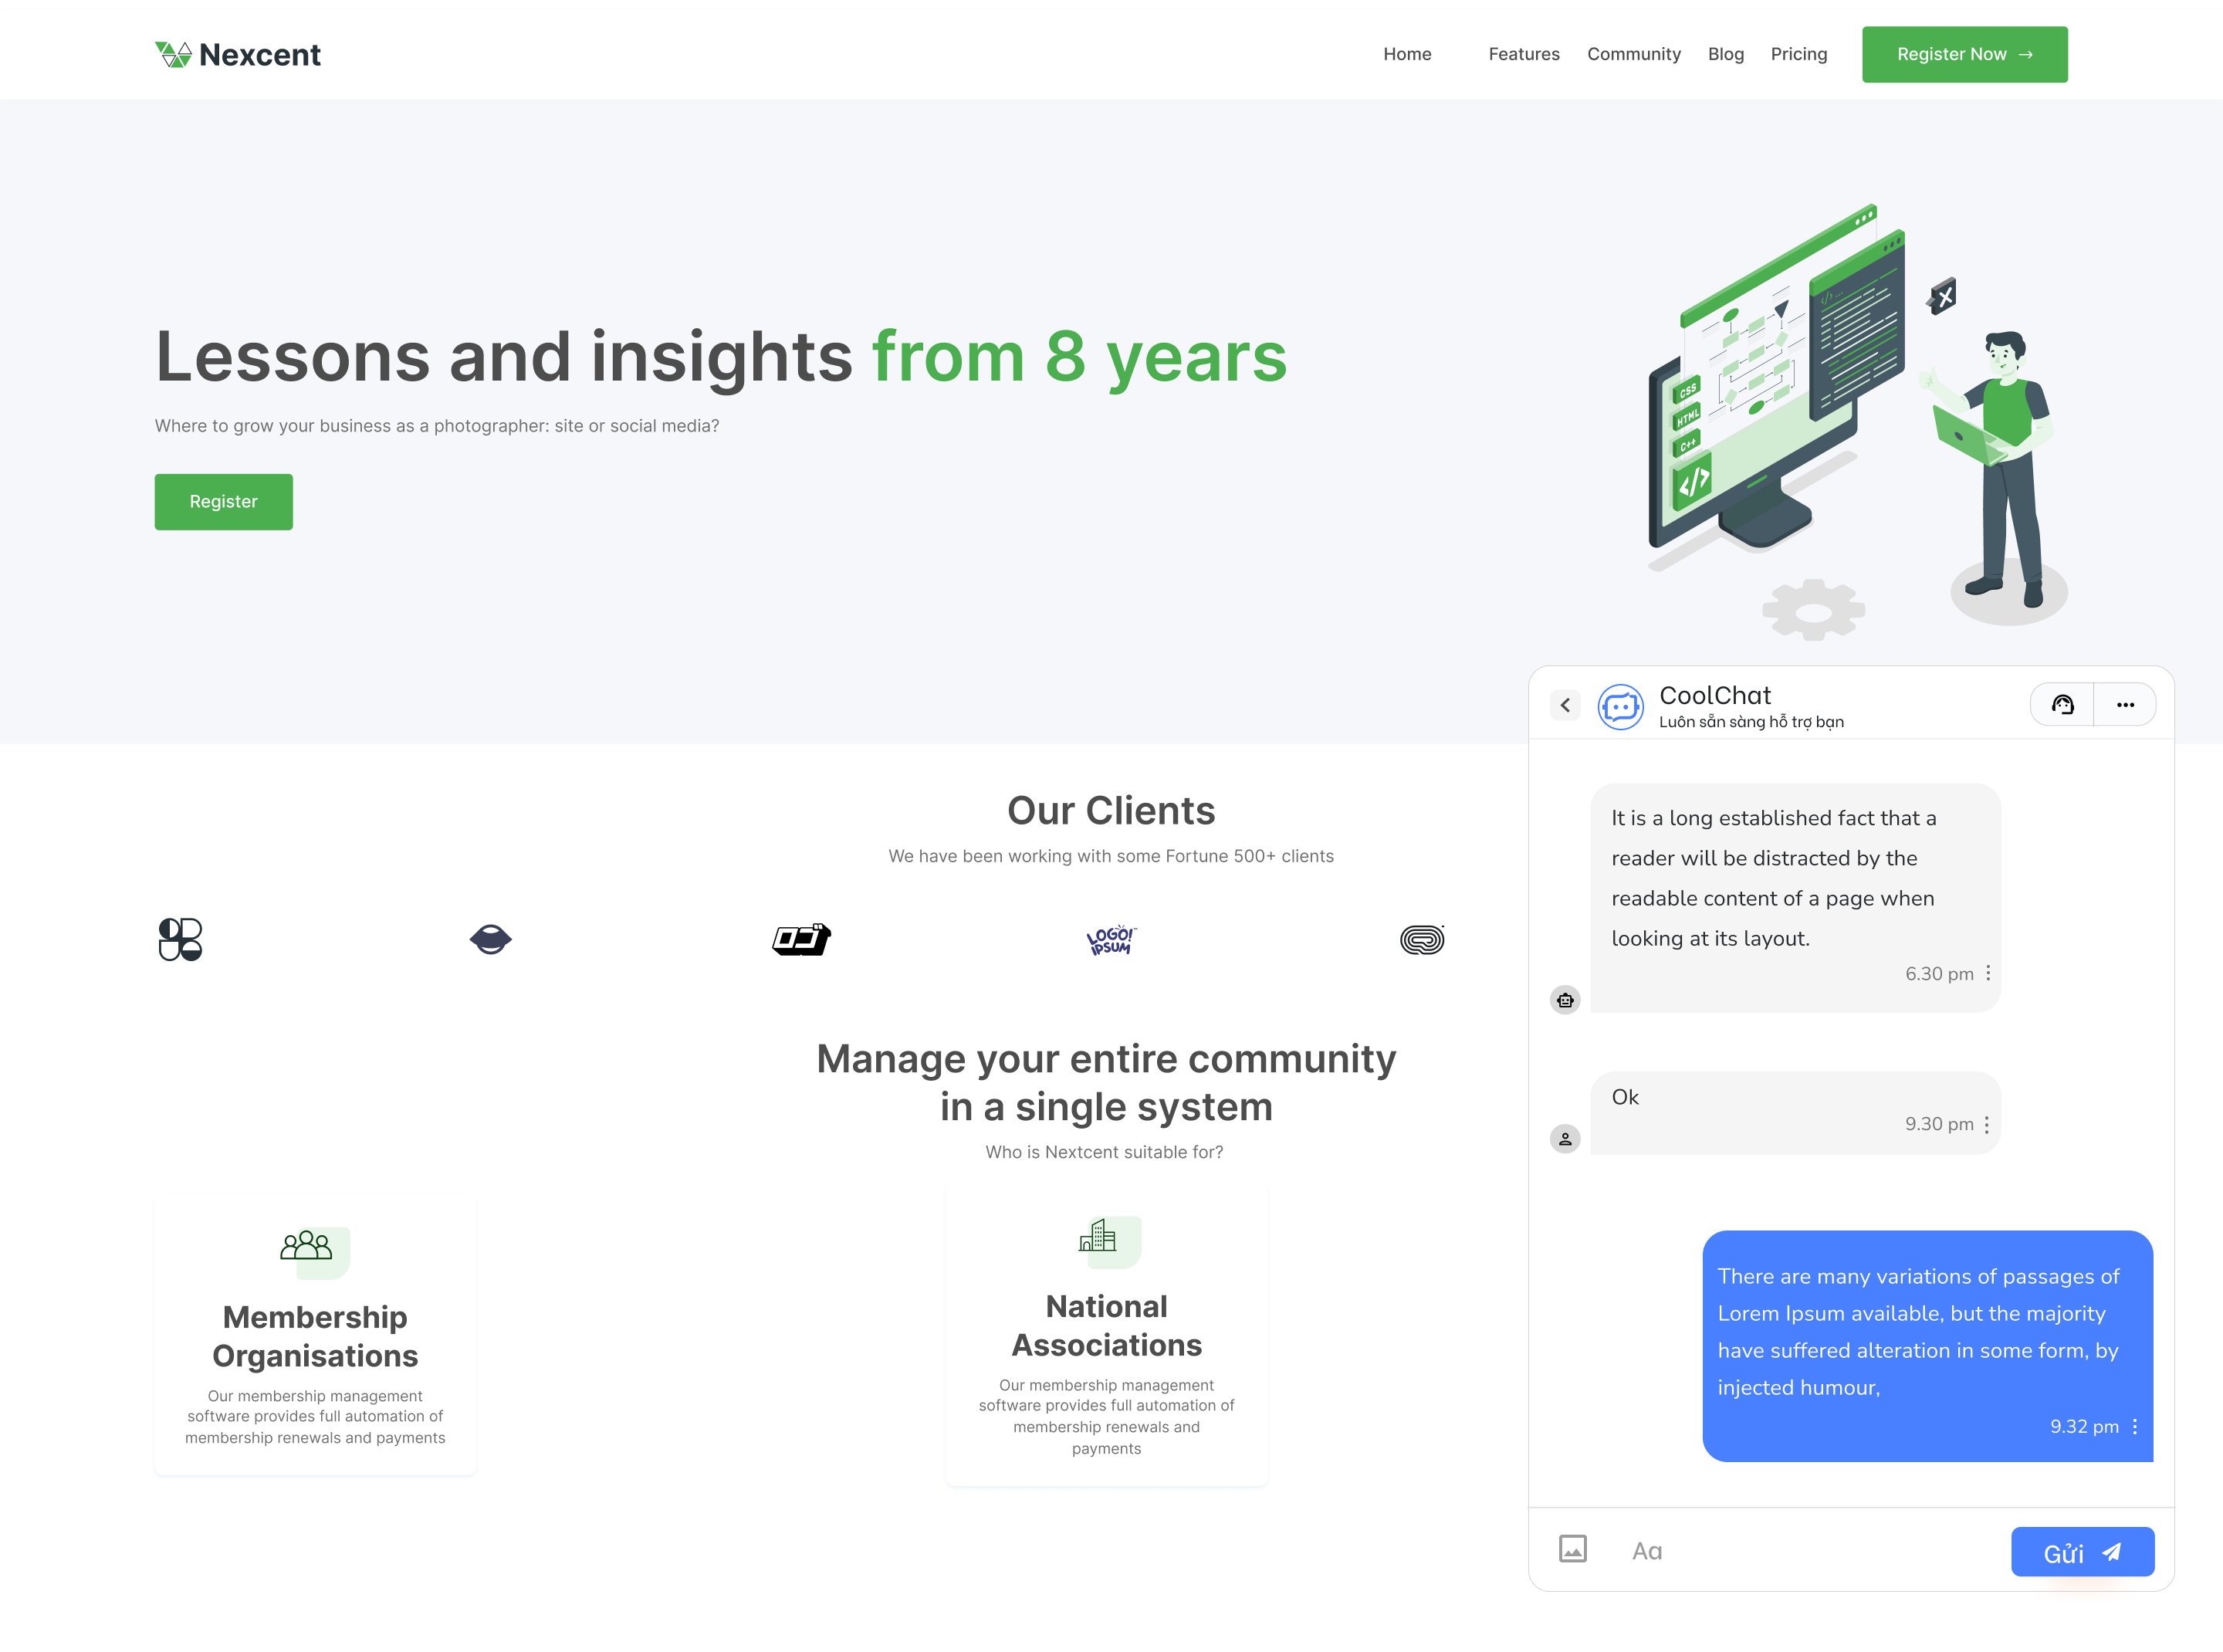
\includegraphics[width=\textwidth]{Figma/customer.png}}
	\vspace{0.5cm}
	\caption{Giao diện phía khách hàng}
	\label{fig:enter-label}
\end{figure}

Khách hàng sẽ sử dụng chatbot thông qua một popup nằm ở góc phải dưới cùng của trang web mà doanh nghiệp tích hợp. Ban đầu nó chỉ là một nút tròn. Khi khách hàng bấm vào thì sẽ bật ra cửa sổ chat, ở đó người dùng có thể nhắn tin, tải ảnh, yêu cầu hỗ trợ và đặt lịch hẹn.

\subsection{Cơ sở dữ liệu}
\begin{figure}[p]
    \thispagestyle{empty}
    \centering
    \rotatebox{90}{
        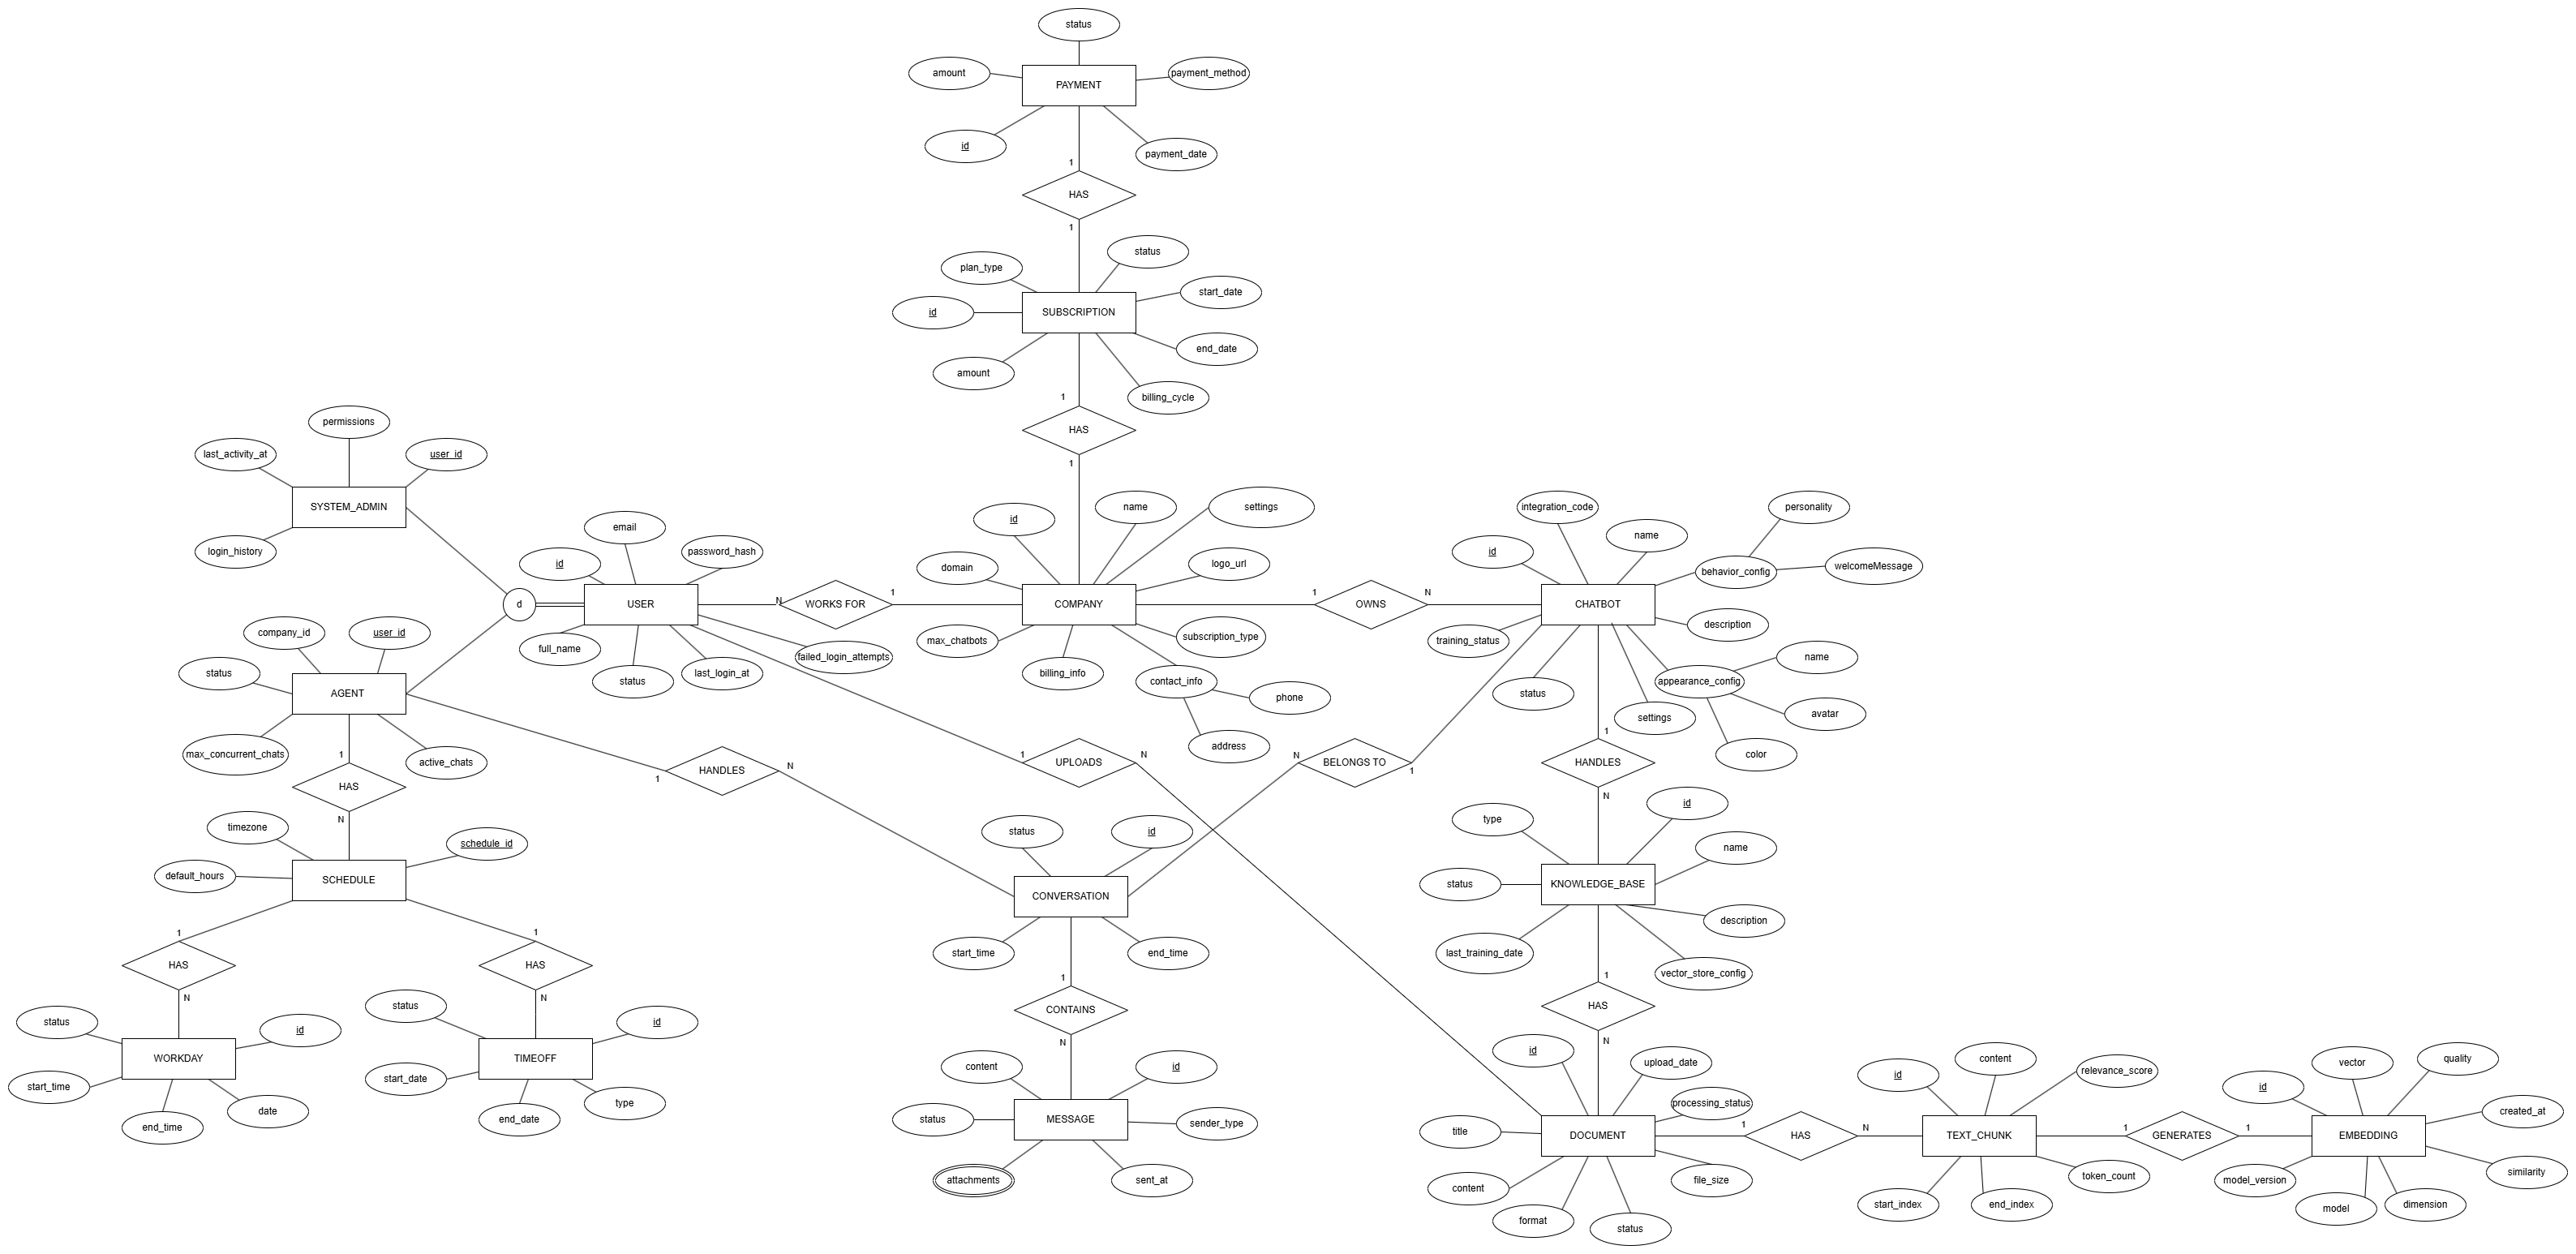
\includegraphics[height=\textwidth, width=\textheight, keepaspectratio]{Dg_System/erd.png}
%\includesvg[height=\textwidth, width=\textheight, keepaspectratio]{Dg_System/ERD.svg}
    }
    \rotatebox{90}{
        \parbox{\textwidth}{
            \centering
            \caption{Biểu đồ ERD hệ thống}
            \label{fig:enter-label}
        }
    }
\end{figure}
\subsubsection{Quản lý công ty và người dùng}
\subsubsubsection{Bảng companies:} Quản lý thông tin các công ty trong hệ thống.

\indent\textbf{Thuộc tính:}
\begin{itemize}
    \item \textbf{id} (UUID): Định danh duy nhất của công ty
    \item \textbf{name} (VARCHAR(255)): Tên công ty
    \item \textbf{domain} (VARCHAR(255)): Tên miền công ty, không được trùng lặp
    \item \textbf{logo\_url} (VARCHAR(512)): Đường dẫn đến logo công ty
    \item \textbf{subscription\_type} (VARCHAR(50)): Loại gói đăng ký (FREE, BASIC, PREMIUM)
    \item \textbf{verification\_status} (VARCHAR(50)): Trạng thái xác thực (PENDING, VERIFIED, REJECTED)
    \item \textbf{contact\_info} (JSONB): Thông tin liên hệ dạng JSON
    \item \textbf{settings} (JSONB): Cấu hình công ty dạng JSON
    \item \textbf{billing\_info} (JSONB): Thông tin thanh toán dạng JSON
    \item \textbf{max\_chatbots} (INTEGER): Số lượng chatbot tối đa được phép tạo
\end{itemize}

\subsubsubsection{Bảng user:} Bảng cơ sở cho tất cả các người dùng trong hệ thống.

\textbf{Thuộc tính:}
\begin{itemize}
    \item \textbf{id} (UUID): Định danh duy nhất của người dùng
    \item \textbf{company\_id} (UUID): Tham chiếu đến công ty
    \item \textbf{email} (VARCHAR(255)): Địa chỉ email đăng nhập, không được trùng lặp
    \item \textbf{password\_hash} (VARCHAR(255)): Mật khẩu đã được mã hóa
    \item \textbf{full\_name} (VARCHAR(255)): Họ và tên đầy đủ
    \item \textbf{last\_login\_at} (TIMESTAMP WITH TIME ZONE): Thời điểm đăng nhập gần nhất
    \item \textbf{failed\_login\_attempts} (INTEGER): Số lần đăng nhập thất bại
    \item \textbf{status} (VARCHAR(50)): Trạng thái tài khoản (ACTIVE, INACTIVE, SUSPENDED)
\end{itemize}

\textbf{Quan hệ:}
\begin{itemize}
    \item Kế thừa từ bảng \texttt{base\_user}
    \item Quan hệ nhiều-một với bảng \texttt{companies}
\end{itemize}

\subsubsubsection{Bảng system\_admins:} Quản lý thông tin quản trị viên hệ thống.

\indent\textbf{Thuộc tính:}
\begin{itemize}
    \item \textbf{id} (UUID): Định danh duy nhất, tham chiếu đến base\_user
    \item \textbf{permissions} (TEXT[]): Mảng các quyền hạn
    \item \textbf{last\_activity\_at} (TIMESTAMP WITH TIME ZONE): Thời điểm hoạt động cuối
    \item \textbf{login\_history} (JSONB): Lịch sử đăng nhập dạng JSON
\end{itemize}

\indent\textbf{Quan hệ:}
\begin{itemize}
    \item Kế thừa từ bảng \texttt{base\_user}
\end{itemize}

\subsubsubsection{Bảng agents:} 

\par Quản lý thông tin nhân viên chăm sóc khách hàng.

\indent\textbf{Thuộc tính:}
\begin{itemize}
    \item \textbf{id} (UUID): Định danh duy nhất, tham chiếu đến base\_user
    \item \textbf{status} (VARCHAR(50)): Trạng thái làm việc (ONLINE, OFFLINE, BUSY)
    \item \textbf{max\_concurrent\_chats} (INTEGER): Số cuộc hội thoại tối đa có thể xử lý
    \item \textbf{active\_chats} (INTEGER): Số cuộc hội thoại đang xử lý
    \item \textbf{availability\_status} (VARCHAR(50)): Trạng thái khả dụng
\end{itemize}

\textbf{Quan hệ:}
\begin{itemize}
    \item Kế thừa từ bảng \texttt{base\_user}
    \item Quan hệ một-một với bảng \texttt{schedules}
\end{itemize}

\subsubsection{Quản lý lịch làm việc}
\subsubsubsection{Bảng schedules: } Quản lý lịch làm việc của nhân viên.

\indent\textbf{Thuộc tính:}
\begin{itemize}
    \item \textbf{id} (UUID): Định danh duy nhất
    \item \textbf{agent\_id} (UUID): Tham chiếu đến nhân viên
    \item \textbf{timezone} (VARCHAR(50)): Múi giờ làm việc
    \item \textbf{default\_hours} (JSONB): Cấu hình giờ làm việc mặc định
\end{itemize}

\textbf{Quan hệ:}
\begin{itemize}
    \item Quan hệ một-một với bảng \texttt{agents}
    \item Quan hệ một-nhiều với bảng \texttt{workdays}
    \item Quan hệ một-nhiều với bảng \texttt{timeoffs}
    \item Kế thừa từ bảng \texttt{base\_entity}
\end{itemize}

\subsubsubsection{Bảng workday: }
Quản lý chi tiết ngày làm việc của nhân viên.

\indent\textbf{Thuộc tính:}
\begin{itemize}
    \item \textbf{id} (UUID): Định danh duy nhất
    \item \textbf{schedule\_id} (UUID): Tham chiếu đến lịch làm việc
    \item \textbf{date} (DATE): Ngày làm việc
    \item \textbf{start\_time} (TIME): Giờ bắt đầu ca làm việc
    \item \textbf{end\_time} (TIME): Giờ kết thúc ca làm việc
    \item \textbf{status} (VARCHAR(50)): Trạng thái ngày làm việc (SCHEDULED, COMPLETED, CANCELLED)
\end{itemize}

\textbf{Quan hệ:}
\begin{itemize}
    \item Quan hệ nhiều-một với bảng \texttt{schedules}
    \item Kế thừa từ bảng \texttt{base\_entity}
\end{itemize}

\subsubsubsection{Bảng timeoff: }Quản lý thông tin nghỉ phép và nghỉ việc của nhân viên.

\indent\textbf{Thuộc tính:}
\begin{itemize}
    \item \textbf{id} (UUID): Định danh duy nhất
    \item \textbf{schedule\_id} (UUID): Tham chiếu đến lịch làm việc
    \item \textbf{start\_date} (DATE): Ngày bắt đầu nghỉ
    \item \textbf{end\_date} (DATE): Ngày kết thúc nghỉ
    \item \textbf{type} (VARCHAR(50)): Loại nghỉ phép (VACATION, SICK\_LEAVE, PERSONAL\_LEAVE)
    \item \textbf{status} (VARCHAR(50)): Trạng thái đơn nghỉ (PENDING, APPROVED, REJECTED)
\end{itemize}

\textbf{Quan hệ:}
\begin{itemize}
    \item Quan hệ nhiều-một với bảng \texttt{schedules}
    \item Kế thừa từ bảng \texttt{base\_entity}
\end{itemize}

\subsubsection{Quản lý Chatbot}

\subsubsubsection{Bảng chatbot: }Quản lý thông tin và cấu hình chatbot.

\indent\textbf{Thuộc tính:}
\begin{itemize}
    \item \textbf{id} (UUID): Định danh duy nhất
    \item \textbf{company\_id} (UUID): Tham chiếu đến công ty sở hữu
    \item \textbf{name} (VARCHAR(255)): Tên chatbot
    \item \textbf{description} (TEXT): Mô tả chức năng
    \item \textbf{status} (VARCHAR(50)): Trạng thái hoạt động
    \item \textbf{training\_status} (VARCHAR(50)): Trạng thái huấn luyện
    \item \textbf{behavior\_config} (JSONB): Cấu hình hành vi
    \item \textbf{appearance\_config} (JSONB): Cấu hình giao diện
    \item \textbf{settings} (JSONB): Thiết lập chung
    \item \textbf{integration\_code} (STRING): Mã nhúng tích hợp
\end{itemize}

\textbf{Quan hệ:}
\begin{itemize}
    \item Quan hệ nhiều-một với bảng \texttt{companies}
    \item Quan hệ một-nhiều với bảng \texttt{knowledge\_bases}
    \item Quan hệ một-nhiều với bảng \texttt{conversations}
    \item Kế thừa từ bảng \texttt{base\_entity}
\end{itemize}

\subsubsubsection{Bảng knowledge\_bases: }Quản lý cơ sở kiến thức của chatbot.

\indent\textbf{Thuộc tính:}
\begin{itemize}
    \item \textbf{id} (UUID): Định danh duy nhất
    \item \textbf{chatbot\_id} (UUID): Tham chiếu đến chatbot
    \item \textbf{name} (VARCHAR(255)): Tên cơ sở kiến thức
    \item \textbf{description} (TEXT): Mô tả nội dung
    \item \textbf{type} (VARCHAR(50)): Loại kiến thức
    \item \textbf{status} (VARCHAR(50)): Trạng thái hoạt động
    \item \textbf{last\_training\_date} (TIMESTAMP WITH TIME ZONE): Thời điểm huấn luyện gần nhất
    \item \textbf{vector\_store\_config} (JSONB): Cấu hình lưu trữ vector
\end{itemize}

\textbf{Quan hệ:}
\begin{itemize}
    \item Quan hệ nhiều-một với bảng \texttt{chatbots}
    \item Quan hệ một-nhiều với bảng \texttt{documents}
    \item Kế thừa từ bảng \texttt{base\_entity}
\end{itemize}

\subsubsubsection{Bảng documents: }Quản lý tài liệu trong cơ sở kiến thức.

\indent\textbf{Thuộc tính:}
\begin{itemize}
    \item \textbf{id} (UUID): Định danh duy nhất
    \item \textbf{knowledge\_base\_id} (UUID): Tham chiếu đến cơ sở kiến thức
    \item \textbf{title} (VARCHAR(255)): Tiêu đề tài liệu
    \item \textbf{content} (TEXT): Nội dung tài liệu
    \item \textbf{format} (VARCHAR(50)): Định dạng file (PDF, DOC, TXT)
    \item \textbf{file\_size} (BIGINT): Kích thước file
    \item \textbf{status} (VARCHAR(50)): Trạng thái xử lý
    \item \textbf{processing\_status} (VARCHAR(50)): Trạng thái xử lý
    \item \textbf{uploaded\_by} (UUID): Tham chiếu đến người tải lên
\end{itemize}

\textbf{Quan hệ:}
\begin{itemize}
    \item Quan hệ nhiều-một với bảng \texttt{knowledge\_bases}
    \item Quan hệ một-nhiều với bảng \texttt{text\_chunks}
    \item Quan hệ nhiều-một với bảng \texttt{base\_user}
    \item Kế thừa từ bảng \texttt{base\_entity}
\end{itemize}

\subsubsection{Xử lý ngôn ngữ tự nhiên}

\subsubsubsection{Bảng text\_chunks: }Quản lý các đoạn văn bản đã được phân đoạn.

\indent\textbf{Thuộc tính:}
\begin{itemize}
    \item \textbf{id} (UUID): Định danh duy nhất
    \item \textbf{document\_id} (UUID): Tham chiếu đến tài liệu gốc
    \item \textbf{content} (TEXT): Nội dung đoạn văn bản
    \item \textbf{start\_index} (INTEGER): Vị trí bắt đầu trong tài liệu
    \item \textbf{end\_index} (INTEGER): Vị trí kết thúc trong tài liệu
    \item \textbf{relevance\_score} (FLOAT): Điểm liên quan
    \item \textbf{token\_count} (INTEGER): Số lượng token
\end{itemize}

\textbf{Quan hệ:}
\begin{itemize}
    \item Quan hệ nhiều-một với bảng \texttt{documents}
    \item Quan hệ một-một với bảng \texttt{embeddings}
    \item Kế thừa từ bảng \texttt{base\_entity}
\end{itemize}

\subsubsubsection{Bảng embeddings: }Quản lý các vector biểu diễn văn bản.

\indent\textbf{Thuộc tính:}
\begin{itemize}
    \item \textbf{id} (UUID): Định danh duy nhất
    \item \textbf{text\_chunk\_id} (UUID): Tham chiếu đến đoạn văn bản
    \item \textbf{vector} (VECTOR(1536)): Vector biểu diễn
    \item \textbf{dimension} (INTEGER): Số chiều vector
    \item \textbf{model} (VARCHAR(255)): Mô hình tạo embedding
    \item \textbf{similarity} (FLOAT): Độ tương đồng
    \item \textbf{quality} (FLOAT): Chất lượng embedding
    \item \textbf{model\_version} (VARCHAR(50)): Phiên bản mô hình
\end{itemize}

\textbf{Quan hệ:}
\begin{itemize}
    \item Quan hệ một-một với bảng \texttt{text\_chunks}
    \item Kế thừa từ bảng \texttt{base\_entity}
\end{itemize}

\subsubsection{Quản lý hội thoại}
\subsubsubsection{Bảng conversations: }

Quản lý các cuộc hội thoại.

\indent\textbf{Thuộc tính:}
\begin{itemize}
    \item \textbf{id} (UUID): Định danh duy nhất
    \item \textbf{chatbot\_id} (UUID): Tham chiếu đến chatbot
    \item \textbf{agent\_id} (UUID): Tham chiếu đến nhân viên
    \item \textbf{status} (VARCHAR(50)): Trạng thái hội thoại
    \item \textbf{start\_time} (TIMESTAMP WITH TIME ZONE): Thời điểm bắt đầu
    \item \textbf{end\_time} (TIMESTAMP WITH TIME ZONE): Thời điểm kết thúc
\end{itemize}

\textbf{Quan hệ:}
\begin{itemize}
    \item Quan hệ nhiều-một với bảng \texttt{chatbots}
    \item Quan hệ nhiều-một với bảng \texttt{agents}
    \item Quan hệ một-nhiều với bảng \texttt{messages}
    \item Kế thừa từ bảng \texttt{base\_entity}
\end{itemize}

\subsubsubsection{Bảng messages:} Quản lý tin nhắn trong hội thoại.

\indent\textbf{Thuộc tính:}
\begin{itemize}
    \item \textbf{id} (UUID): Định danh duy nhất
    \item \textbf{conversation\_id} (UUID): Tham chiếu đến cuộc hội thoại
    \item \textbf{content} (TEXT): Nội dung tin nhắn
    \item \textbf{sender\_type} (VARCHAR(50)): Loại người gửi
    \item \textbf{sent\_at} (TIMESTAMP WITH TIME ZONE): Thời điểm gửi
    \item \textbf{status} (VARCHAR(50)): Trạng thái tin nhắn
    \item \textbf{attachments} (JSONB): Các tệp đính kèm
\end{itemize}

\textbf{Quan hệ:}
\begin{itemize}
    \item Quan hệ nhiều-một với bảng \texttt{conversations}
    \item Kế thừa từ bảng \texttt{base\_entity}
\end{itemize}

